\documentclass[12pt,letterpaper]{article}
%\usepackage{preamble}

%\ProvidesPackage{preamble}

\usepackage{fullpage}
\usepackage[top=2cm, bottom=4.5cm, left=2.5cm, right=2.5cm]{geometry}
\usepackage{amsmath,amsthm,amsfonts,amssymb,amscd}
\usepackage{lastpage}
\usepackage{enumerate}
\usepackage{fancyhdr}
\usepackage{mathrsfs}
\usepackage{xcolor}
\usepackage{graphicx}
\usepackage{listings}
\usepackage{hyperref}
\usepackage{enumitem}
\usepackage{float}
\usepackage{fancyvrb}
\usepackage{color,soul}
\sethlcolor{lightgray}
 \usepackage{subfigure}
 \usepackage{textcomp}
\usepackage{siunitx}

\usepackage{graphicx}
\usepackage{array}

\usepackage[T1]{fontenc}
\usepackage[numbered,framed]{matlab-prettifier}
\hypersetup{%
  colorlinks=true,
  linkcolor=blue,
  linkbordercolor={0 0 1}
}

\let\ph\mlplaceholder % shorter macro
\lstMakeShortInline"

\lstset{
  style              = Matlab-editor,
  basicstyle         = \mlttfamily \small,
  escapechar         = ",
  mlshowsectionrules = true,
  xleftmargin=.01\textwidth, xrightmargin=.01\textwidth
}

\graphicspath{{./problem1_images}}

\pagestyle{fancyplain}
\headheight 35pt
\lhead{\userID}
\chead{\textbf{\Large Project \hwnumber}}
\rhead{\course \\ \today}
\lfoot{}
\cfoot{}
\rfoot{\small\thepage}
\headsep 1.5em




%%%%%%%%%%%%%%%%%%%%%%%%%%%%%%%%%%%%%%%%%%
%%%% Edit These for yourself
%%%%%%%%%%%%%%%%%%%%%%%%%%%%%%%%%%%%%%%%%%
\newcommand\course{Econ 672}
\newcommand\hwnumber{5}
\newcommand\userID{Ziming Huang}
\newenvironment{alphaparts}[0]{%
  \begin{enumerate}[label=\textbf{\Alph*}]
}{\end{enumerate}}


\begin{document}

\section*{Exercise 1-Local Variance}
  \begin{enumerate}[label=\textbf{(\Alph*)}]
%----A-----
\item We can estimate local variance by using this estimator:
$$\hat{c}_{i_t}(t)=\frac{1}{2k_n+1}\sum_{j=-k_n}^{k_n}(r_{i_{t+j}}^c)^2$$
If the jump interval $i_t$ falls in the begin or end of market hour, we can adjust our estimator as:
$$\hat{c}_{i_t}(t)=\frac{1}{J_1-J_2+1}\sum_{j=-J_2}^{J_1}(r_{i_{t+j}}^c)^2$$
with

$$J_2=max(1,i-k_n)$$
$$J_1=min(k_n+i,n)$$

where $i$ is the number of interval intraday that jump time falls in, $n$ is the number of daily observe interval, $k_n$ is the half length of estimate windows.\\

The following is graph of the local variance estimator for PG and DIS on January 3, 2007. 
 \begin{figure}[H]
	\subfigure{
		\begin{minipage}[l]{1\linewidth}
			\centering
			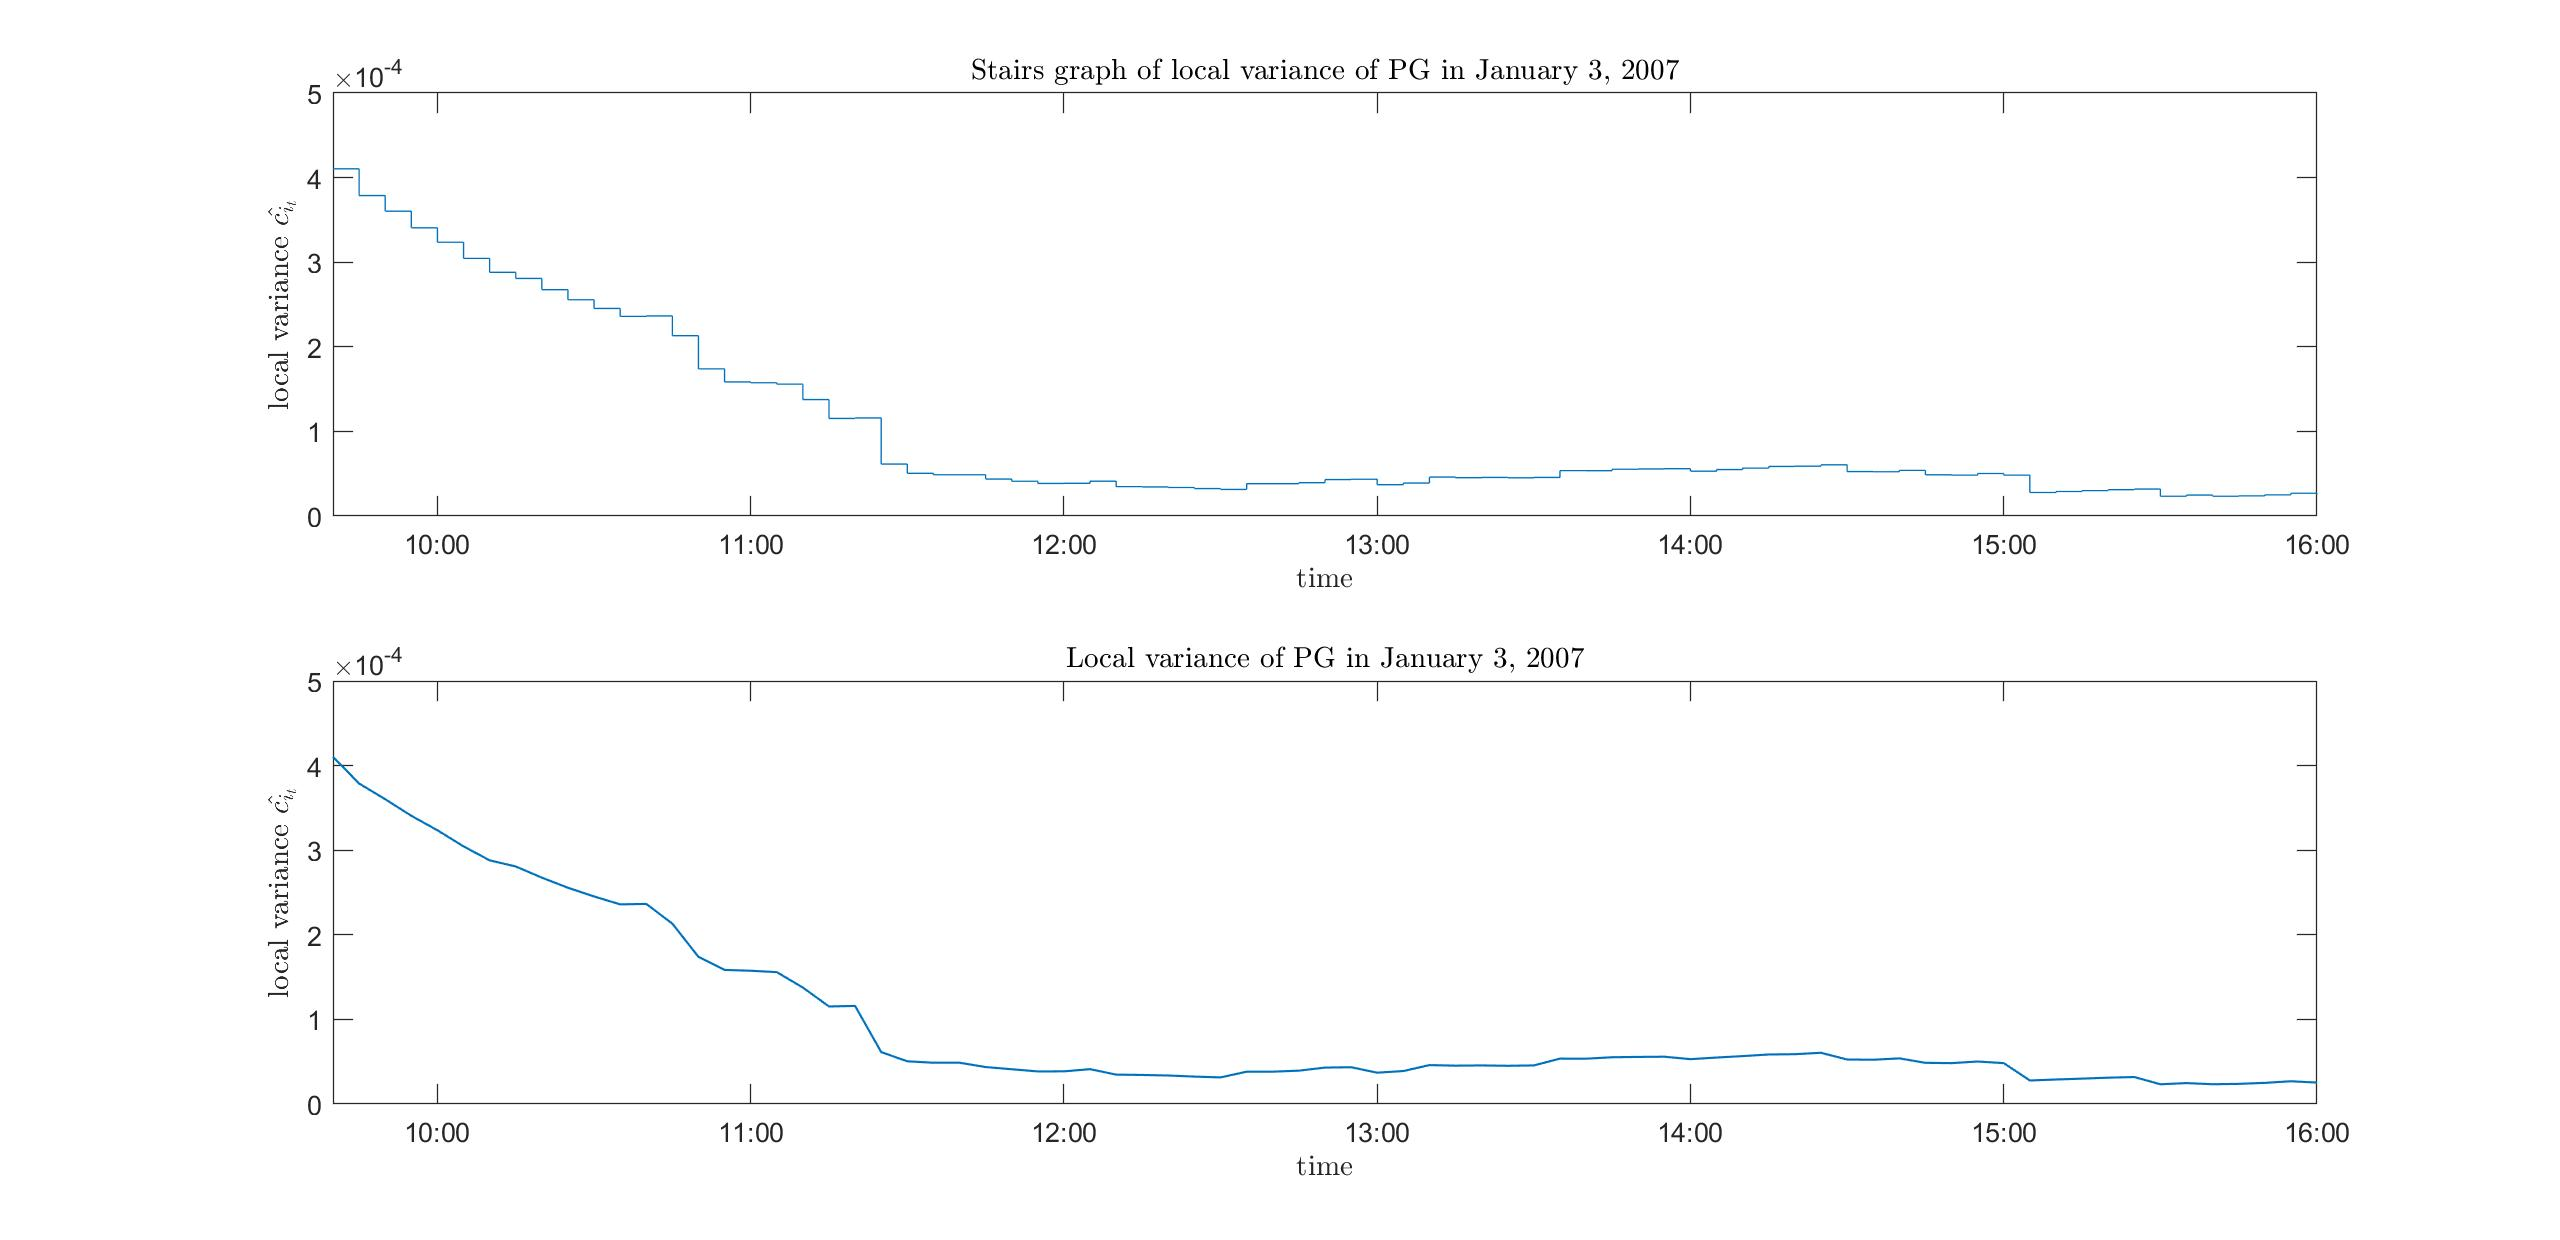
\includegraphics[width=8cm]{figures/1A_PG.jpg}
			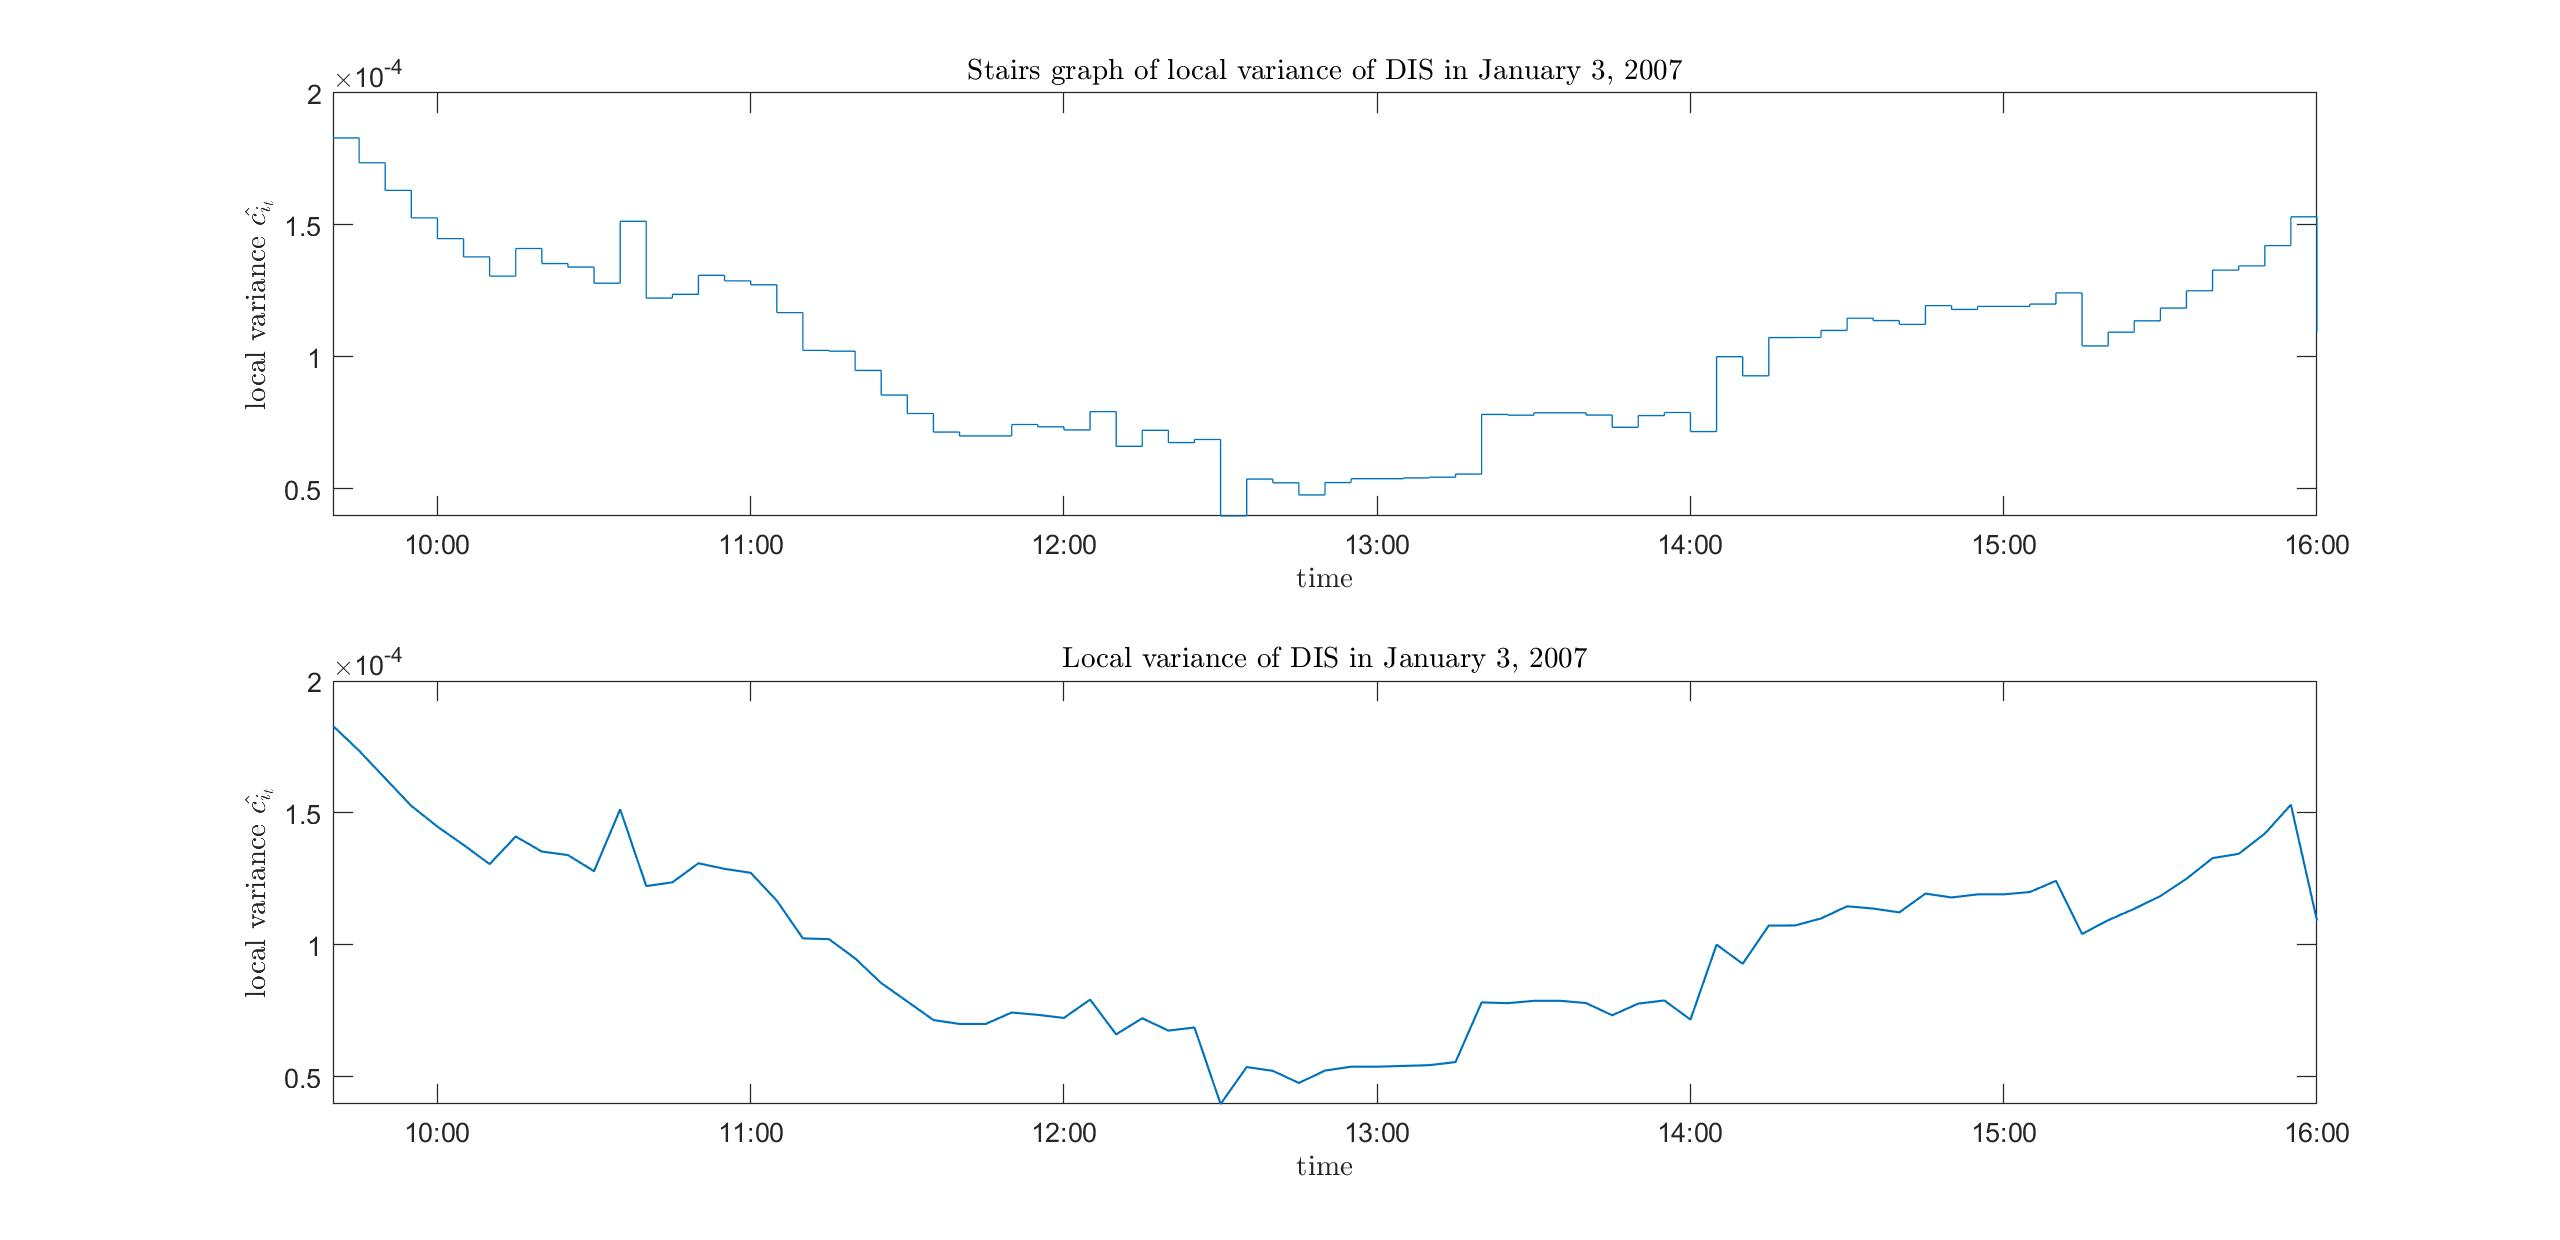
\includegraphics[width=8cm]{figures/1A_DIS.jpg}
		\end{minipage}
	}
	\centering
	\caption{Estimated Local Variance of PG and DIS on January 3, 2007}
\end{figure}

From the graphs we can find the daily local variance shows a U-shape pattern (this is much more obvious in DIS' graph): at the beginning of market hour, the local variance is very high; as the deal goes on, the local variance decreases and always reach its lowest point at the middle of market hour; in the latter part of market hour, the local variance shows a increasing trend. 

As for the value of local variance, we can find DIS' local variance is much larger than the PG's, which mean the volatility of DIS' log-returns will experience larger fluctuations. 

\item We use this estimator to estimate the average local variance for each interval:
$$\bar{\hat{c_i}}=\frac{1}{T}\sum_{t=1}^{T}\hat{c_{i_t}}$$
for $i=1,2,\dots n.$
The following is graph of the local variance estimator for PG and DIS on January 3, 2007. 
 \begin{figure}[H]
	\subfigure{
		\begin{minipage}[l]{1\linewidth}
			\centering
			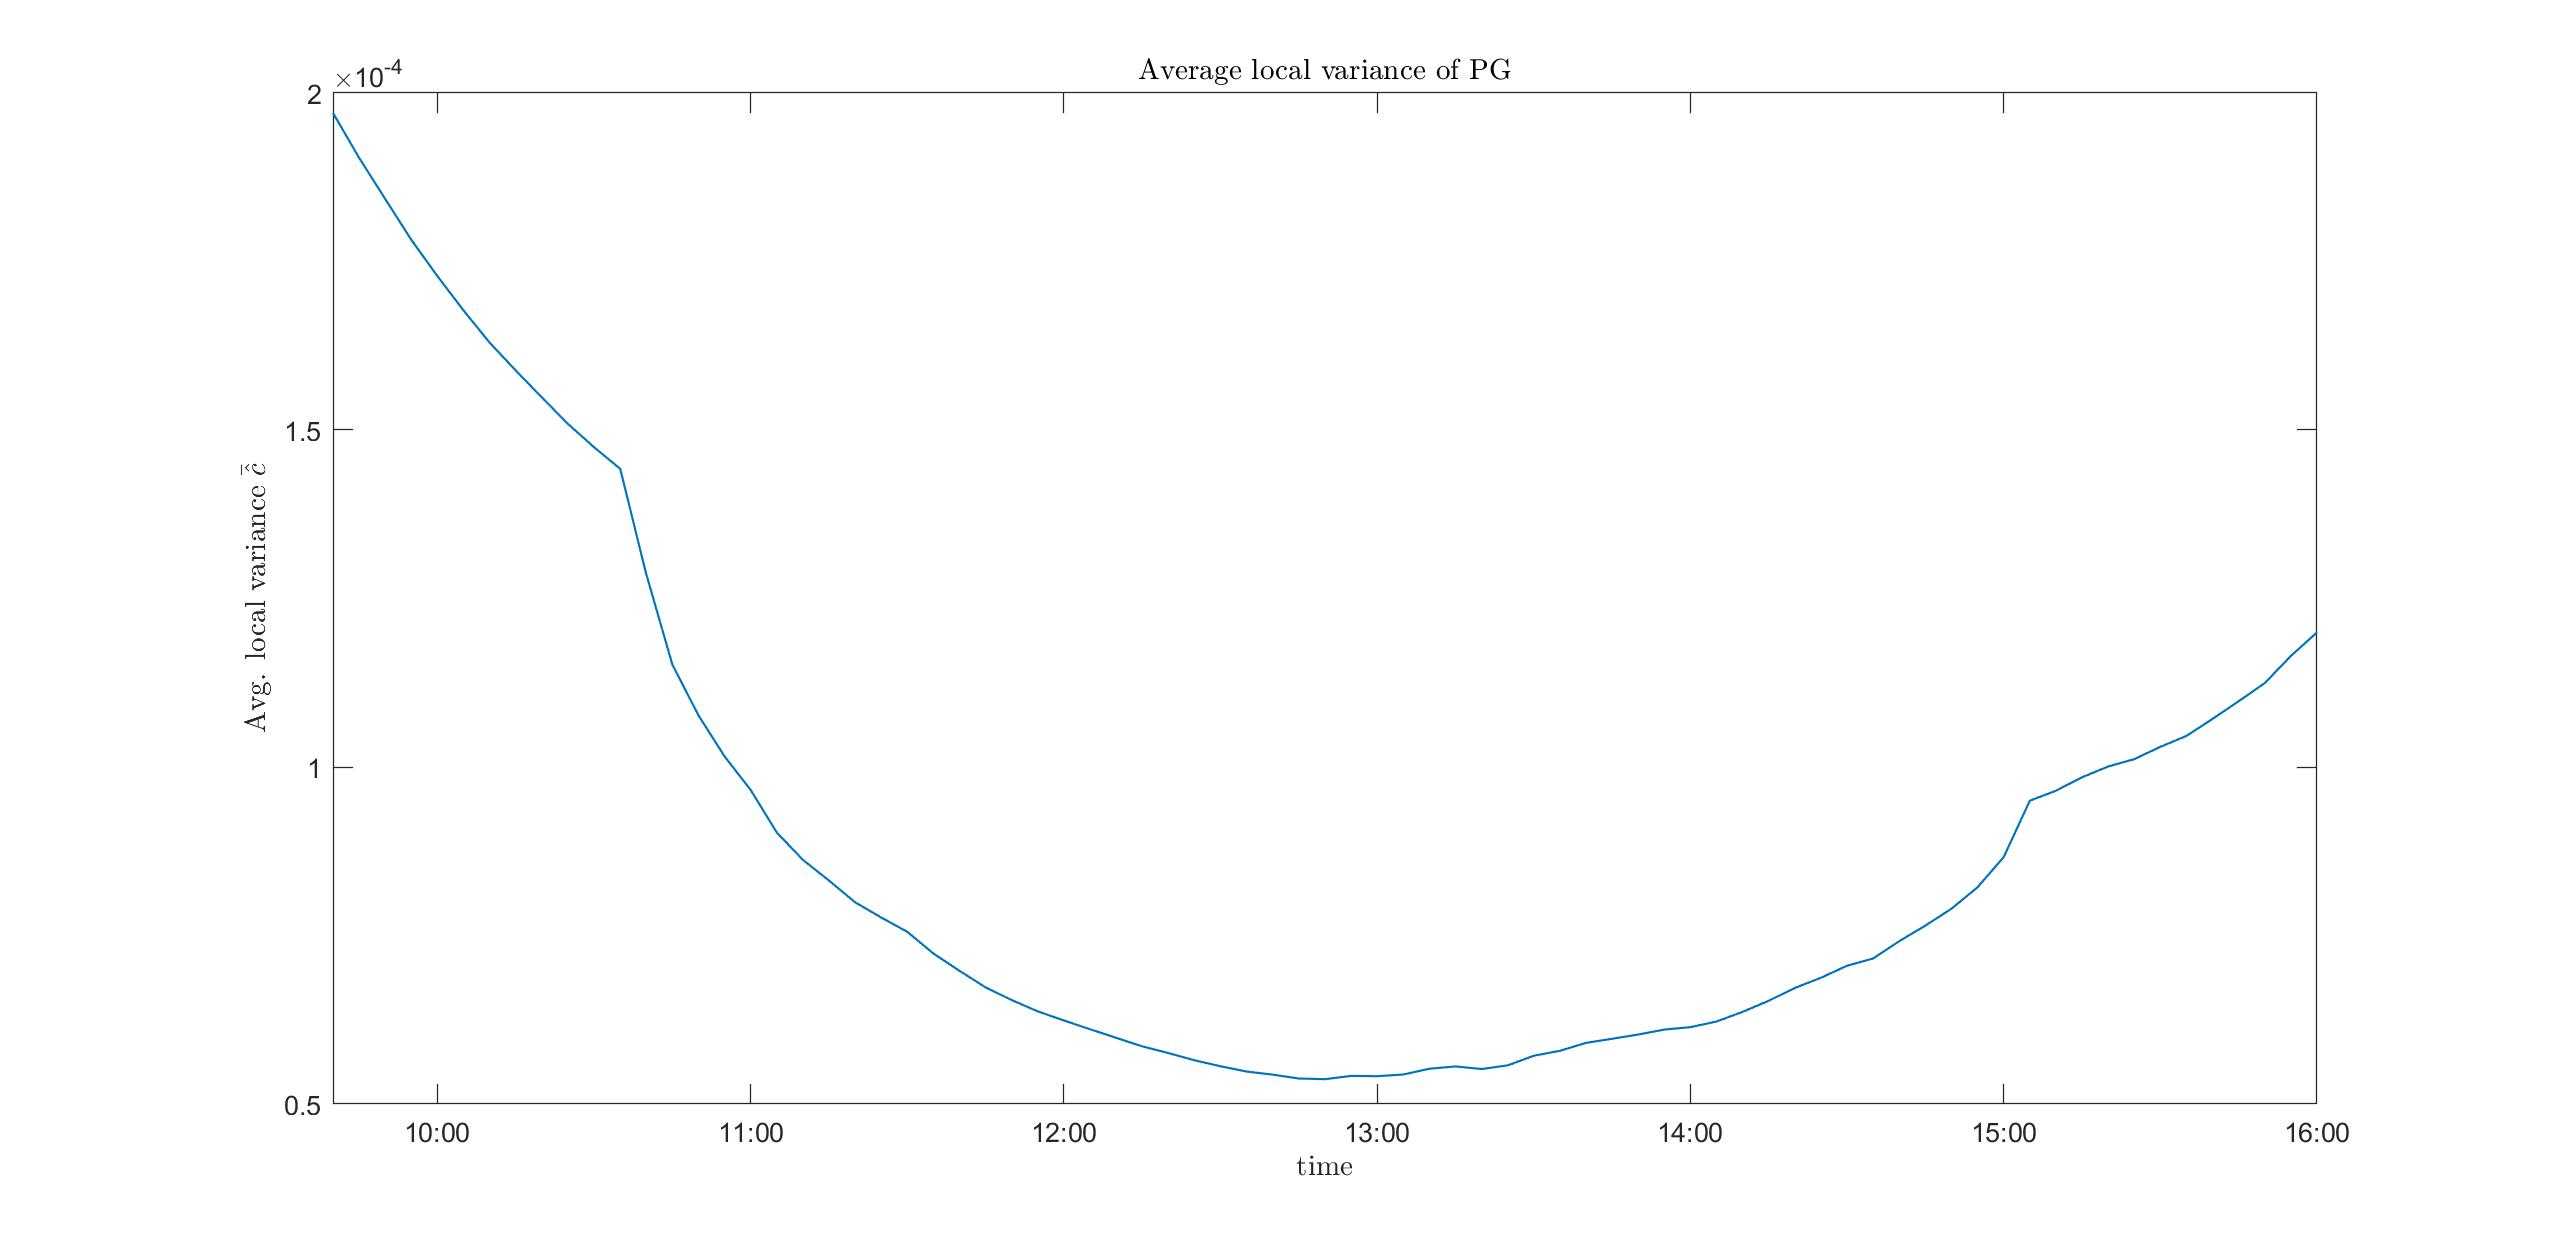
\includegraphics[width=3in]{figures/1B_PG.jpg}
			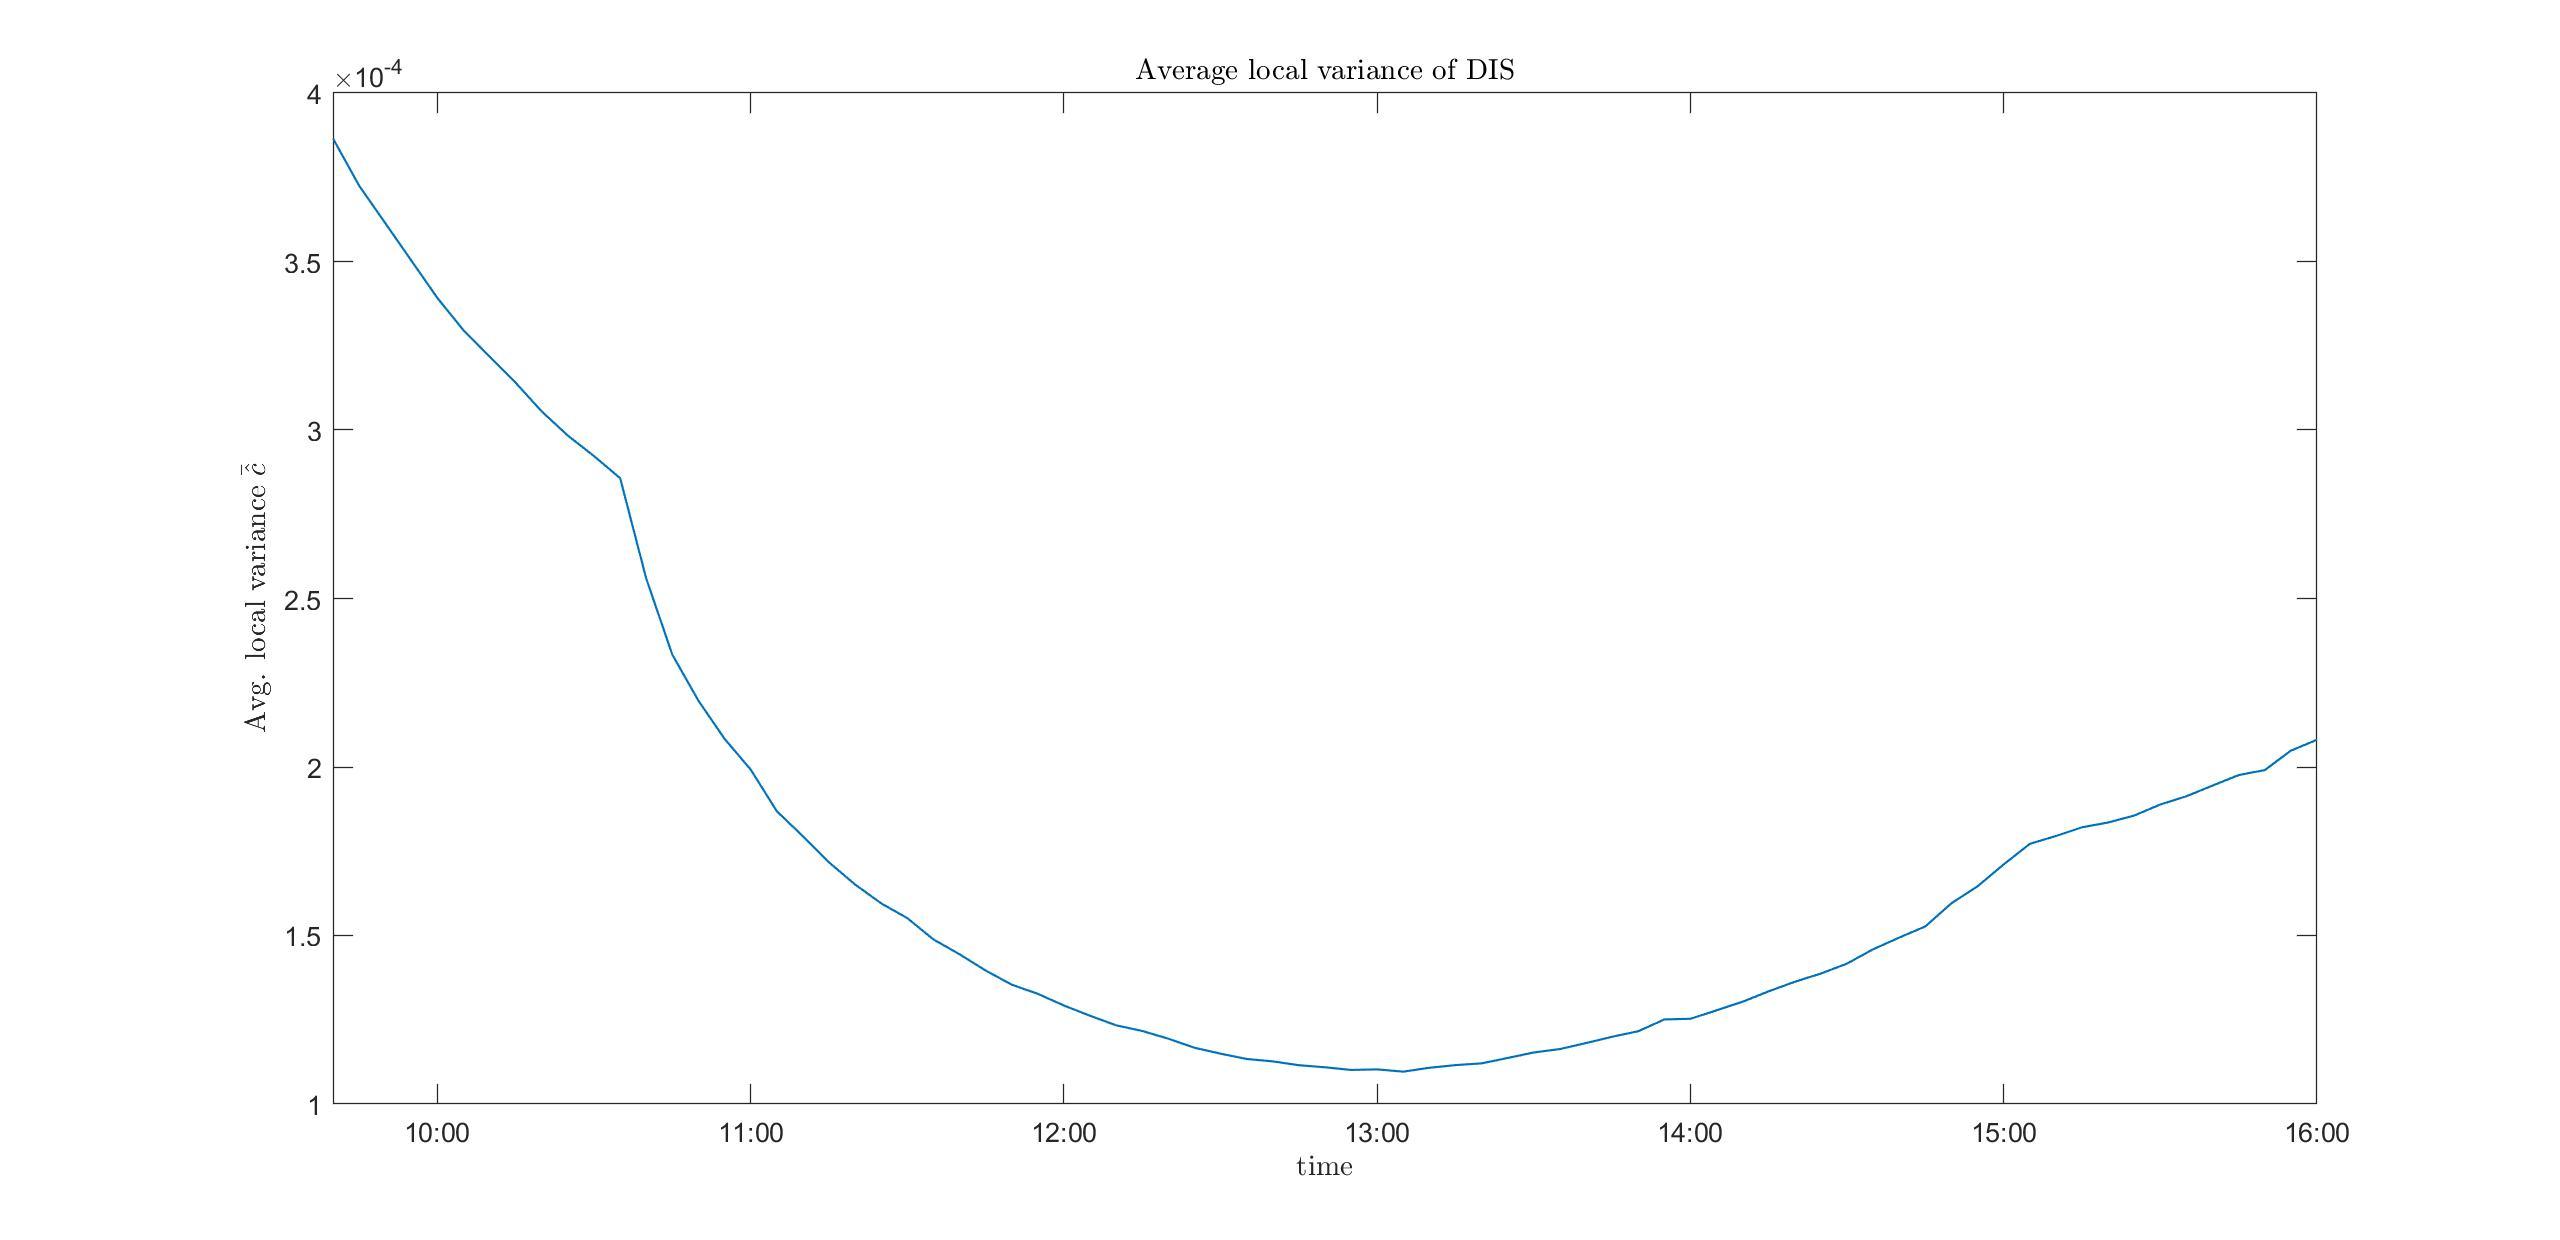
\includegraphics[width=3in]{figures/1B_DIS.jpg}
		\end{minipage}
	}
	\centering
	\caption{Estimated Average Local Variance of PG and DIS}
\end{figure}

After taking average of the local variance throughout all observe time, the U-shape pattern are much clear in for PG and DIS' local variance. From the graphs we can see, the curve shape of these two stocks are very similar, the volatility of DIS is bigger than PG's.\\


The \textbf{MATLAB} code:

Function of Local Variance
   \lstinputlisting{functions/local_var.m}
Scripts of Q1
\lstinputlisting{scripts/ex5_Q1_PG.m}

\end{enumerate}
 

\newpage

%---------------------------------------------

\section*{Exercise 2-Jumps in the Variance}
  \begin{enumerate}[label=\textbf{(\Alph*)}]
%---A---
\item To estimate the volatility before jump $\hat{c}_{i_t}^-$, we use:
$$\hat{c}_{i_t}^-=\frac{1}{i-J_2}\sum_{j=-J_2}^{i-1}(r_{i_{t+j}}^c)^2$$
with $J_2=max(1,i-k_n)$, $i=2,3,\dots n$.

To estimate the volatility before jump $\hat{c}_{i_t}^+$, we use:
$$\hat{c}_{i_t}^+=\frac{1}{J_1-i}\sum_{j=i+1}^{J_1}(r_{i_{t+j}}^c)^2$$
with $J_1=min(k_n+i,n)$, $i=1,2,\dots n-1$.

To measure the magnitude of the jump return, we use absolute value of jump returns:
$$M_{r_{t,i_t}^d}=|r_{t,i_t}^d|$$
with $i=2,3,\dots n$.

The following is graph of $\hat{c}_{i_t}^-$, $\hat{c}_{i_t}^+$ and $|r_{t,i_t}^d|$ of PG and DIS.

 \begin{figure}[H]
	\subfigure{
		\begin{minipage}[l]{1\linewidth}
			\centering
			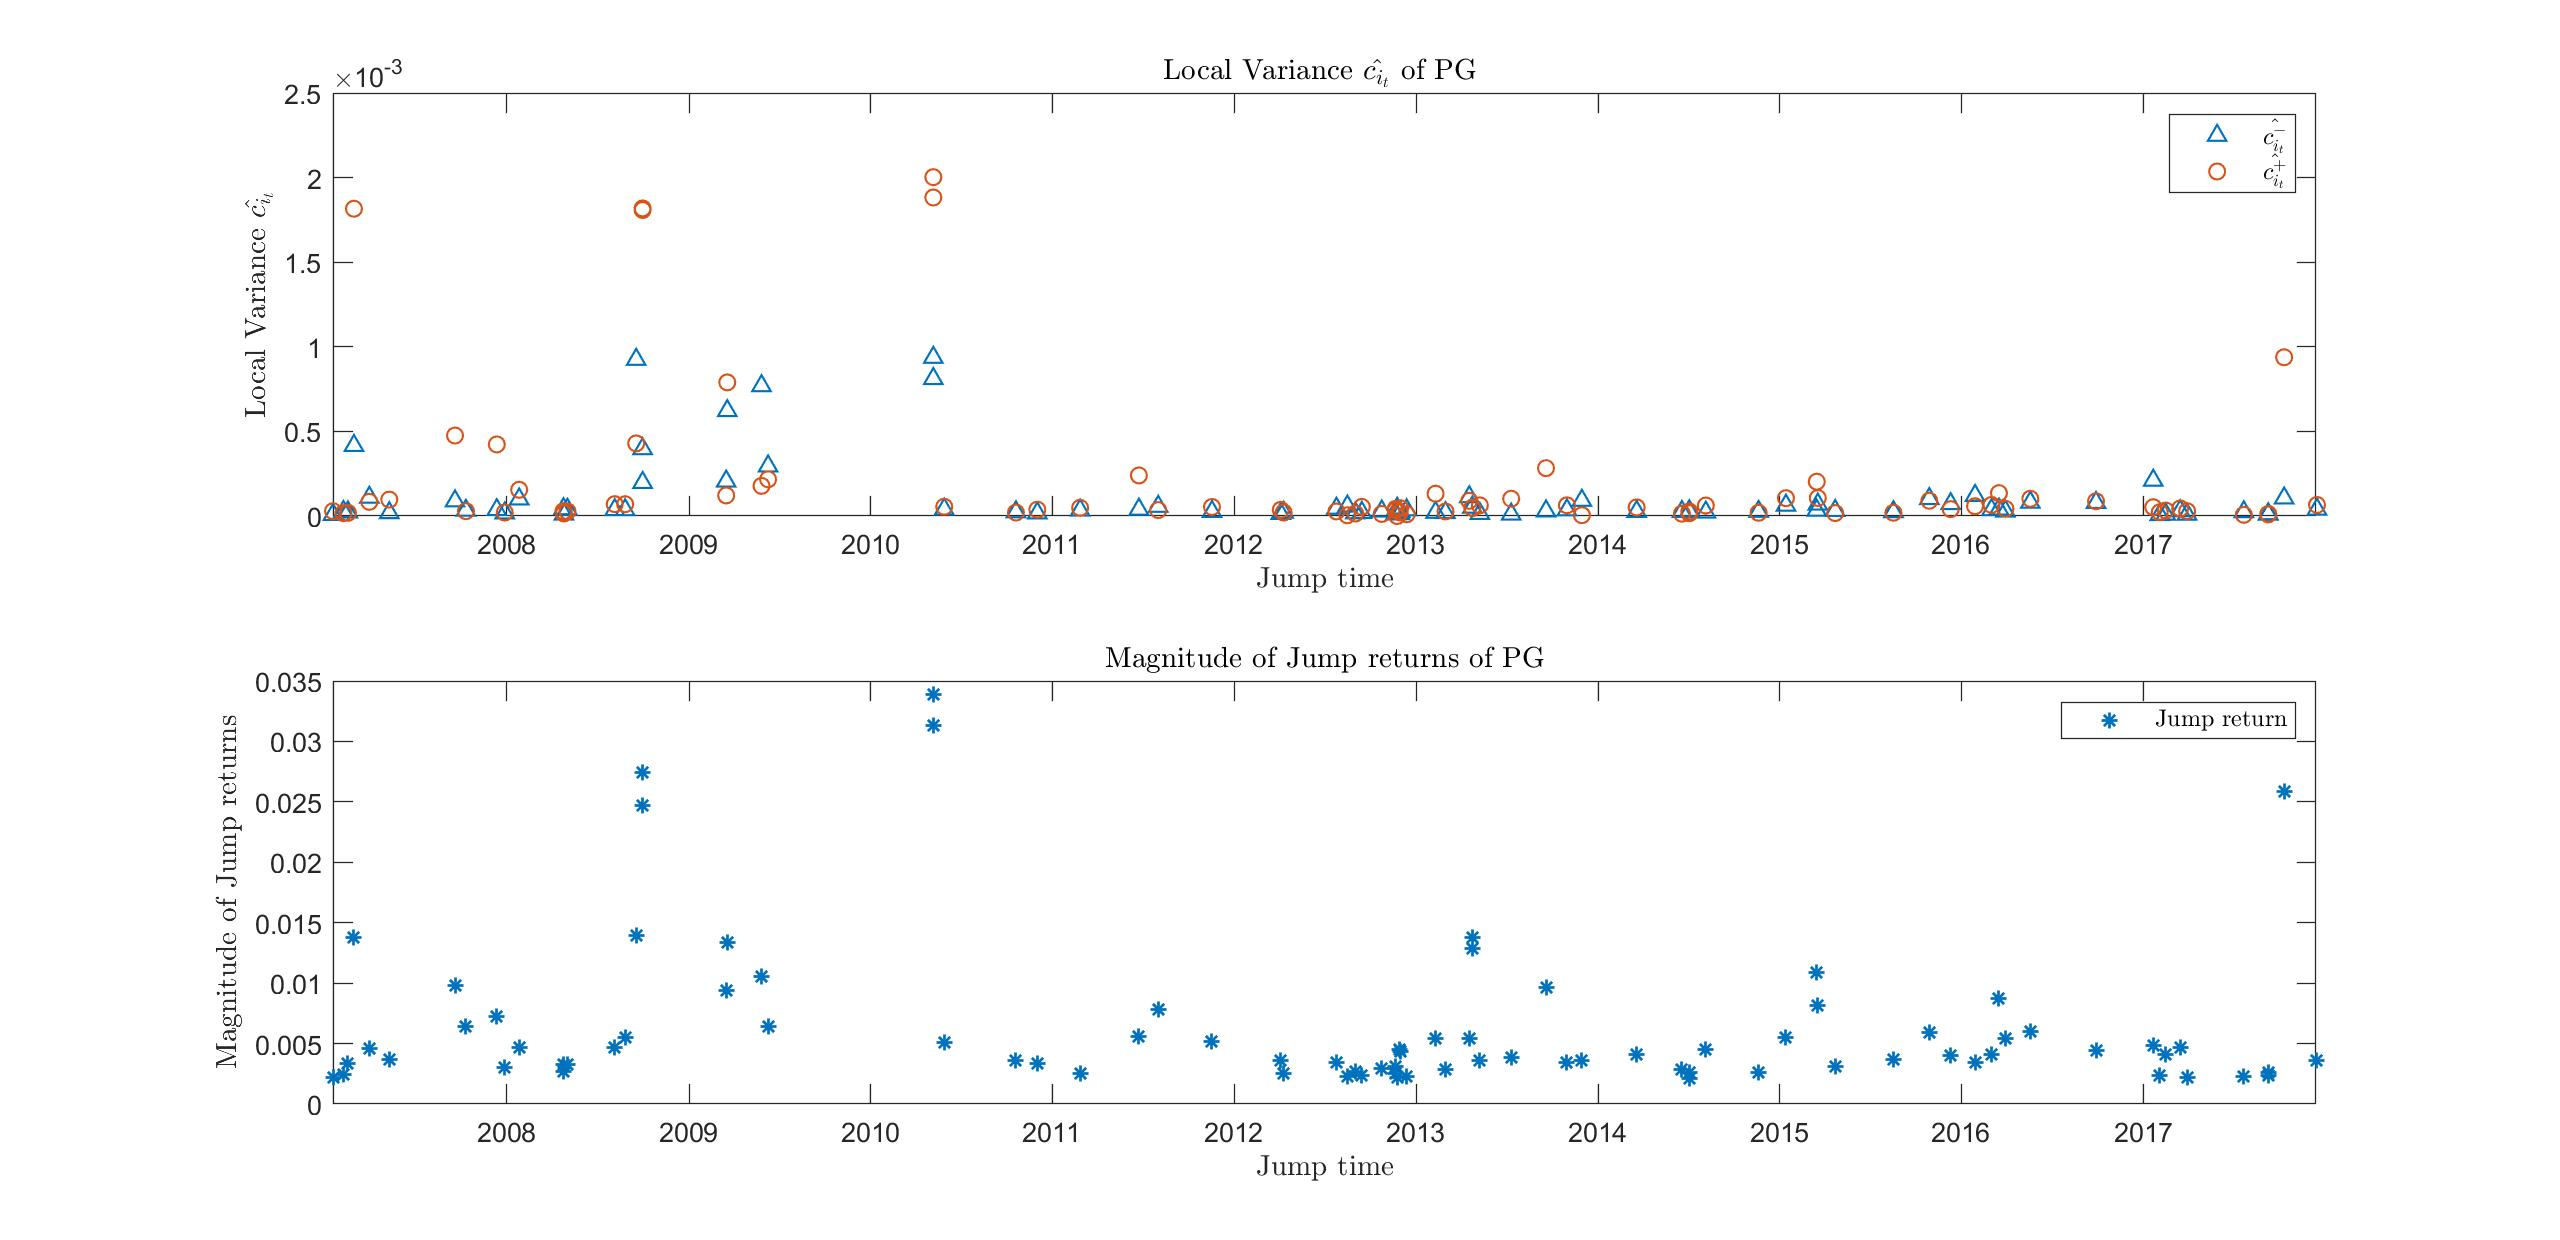
\includegraphics[width=15cm]{figures/2A_PG.jpg}
			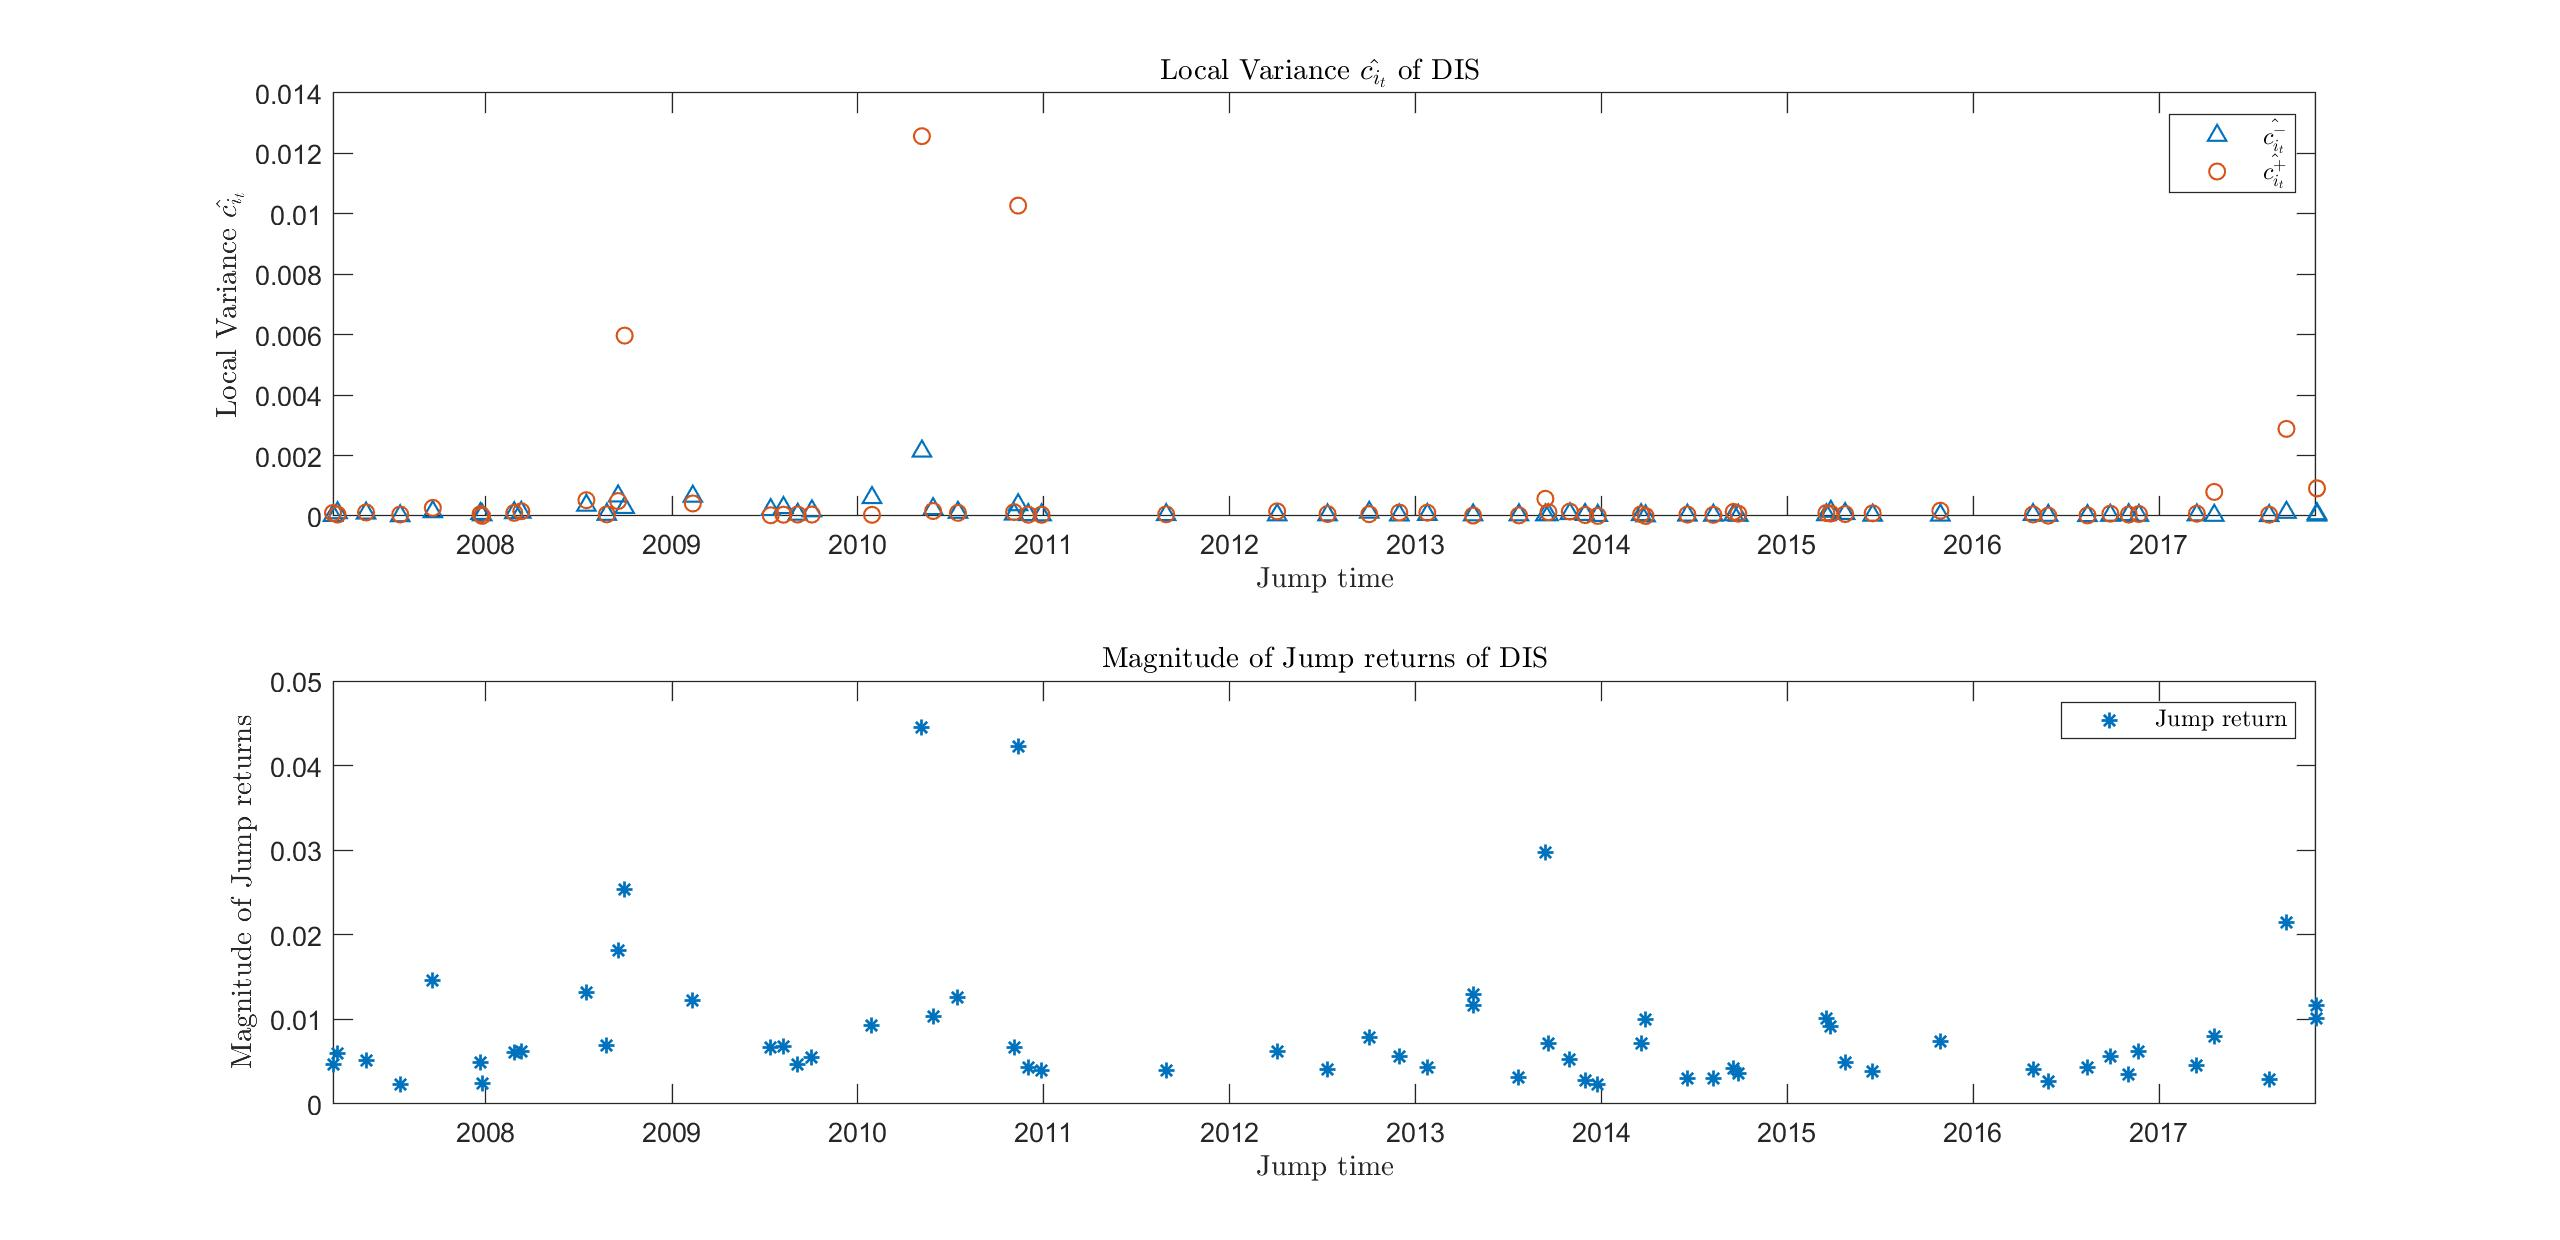
\includegraphics[width=15cm]{figures/2A_DIS.jpg}
		\end{minipage}
	}
	\centering
	\caption{ $\hat{c}_{i_t}^-$, $\hat{c}_{i_t}^+$ and $|r_{t,i_t}^d|$ of PG and DIS}
\end{figure}

From these graphs, we can detect the trading time with large magnitude of jump returns is consistent with the time when the difference of $\hat{c}_{i_t}^-$ and $\hat{c}_{i_t}^+$ is large, which indicates a jump local variance may exist. This finding may give us a method to detect the jump volatility in stock's returns: if there is a large magnitude of stock return in the stock price, then there is a high probability that the volatility is experiencing a jump. 

%-b

\item 
\begin{enumerate}[label=(\roman*)]
	\item To create the confidence interval of left and right local variance, we can use bootstrap method. In order to simplify the programming, we here just focus on those jumps fall in the middle of market hour. This simplification should be reasonable since about 95\% jumps occur in the middle of market hour and the accuracy estimates for the beginning and end interval's local variance are undesirable due to limited available data. \\

    The follows are the graphs of jump local variance and its confidence interval of PG and DIS.

 \begin{figure}[H]
	\subfigure{
		\begin{minipage}[l]{1\linewidth}
			\centering
			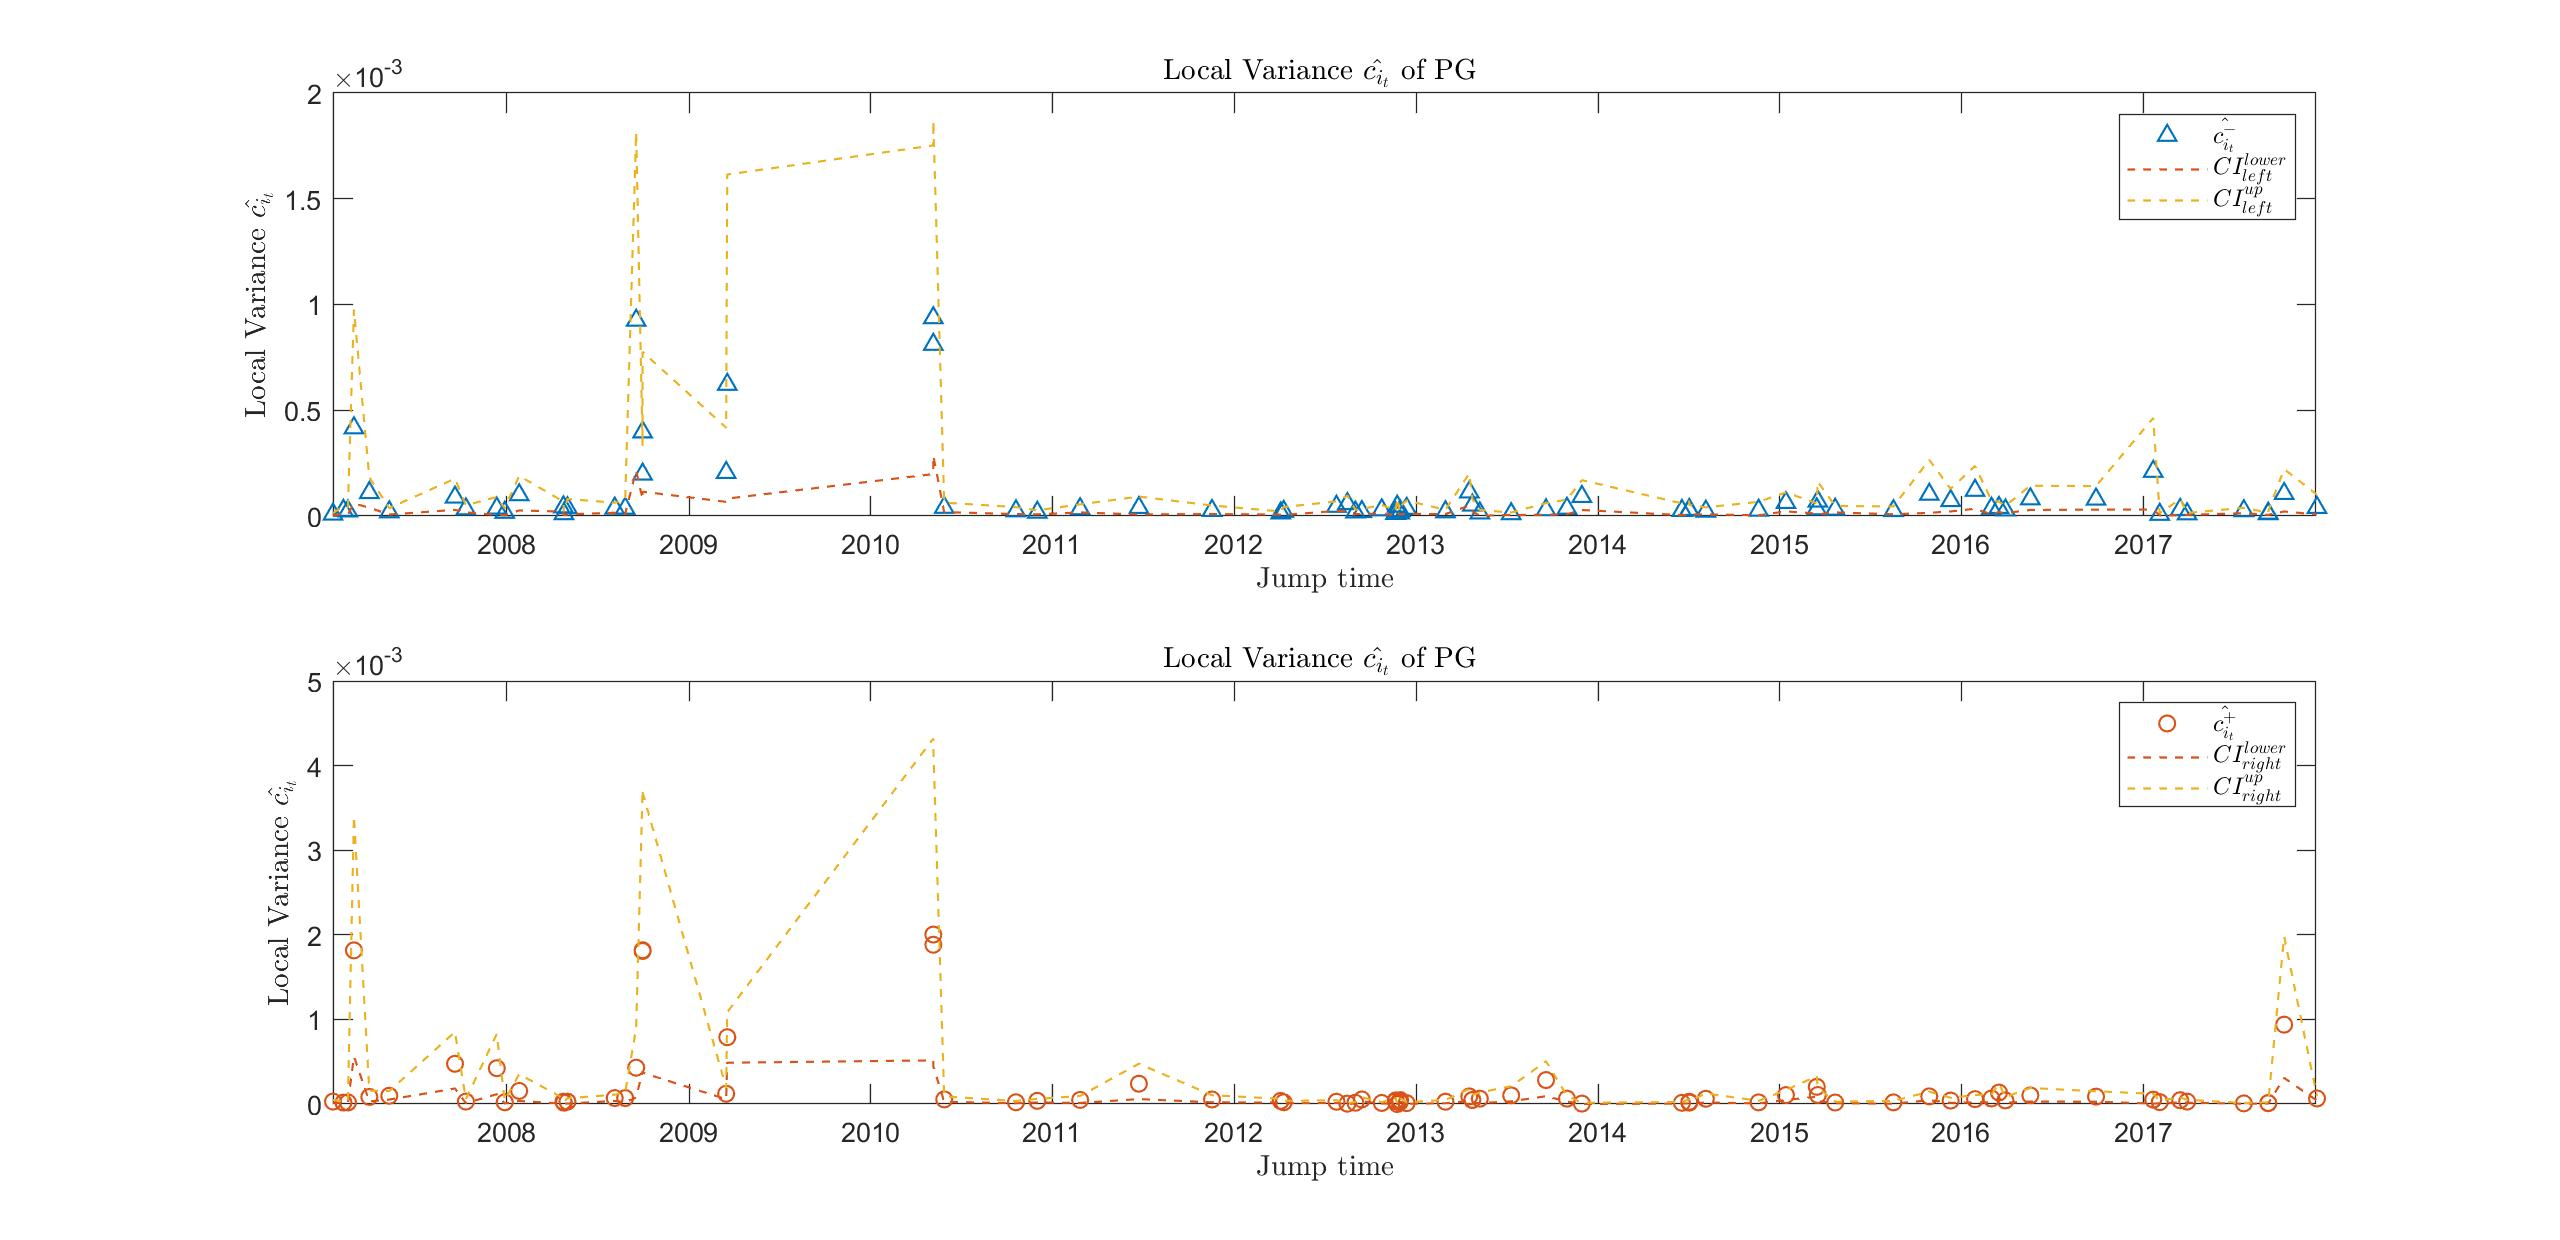
\includegraphics[width=15cm]{figures/2B_PG_1.jpg}
			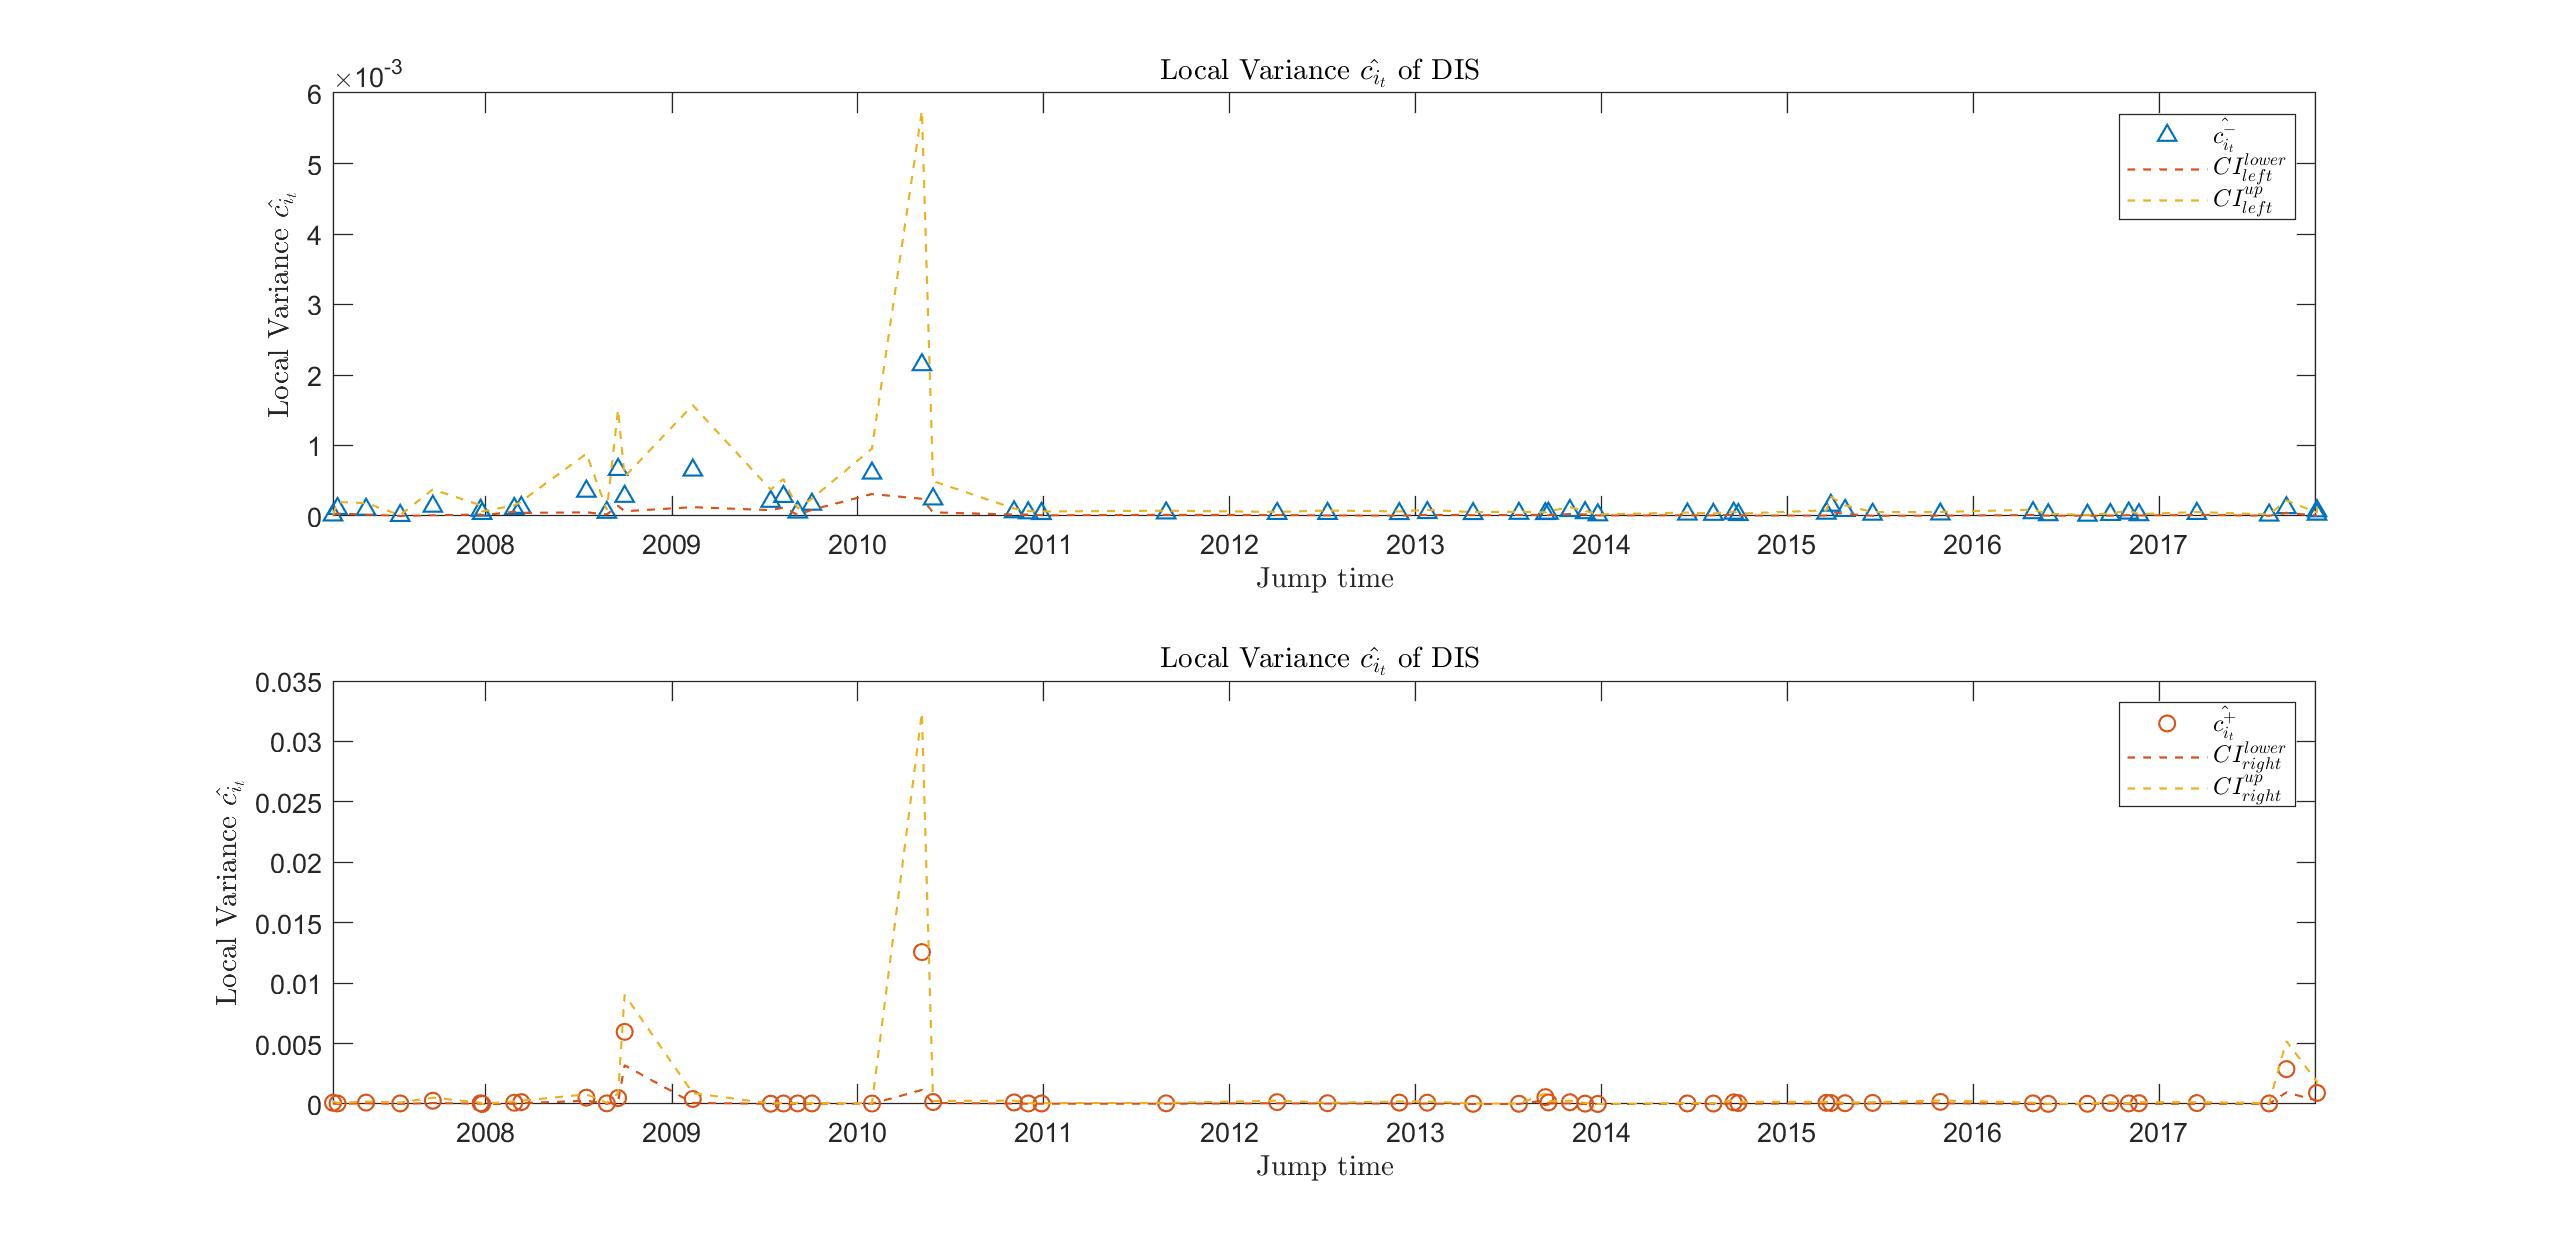
\includegraphics[width=15cm]{figures/2B_DIS_1.jpg}
		\end{minipage}
	}
	\centering
	\caption{ $\hat{c}_{i_t}^-$, $\hat{c}_{i_t}^+$ and its confidence interval of PG and DIS}
\end{figure}

  The first and third graphs are the confidence interval of left limit local variance $\hat{c}_{i_t}^-$ and the second and fourth  graphs are the confidence interval of left limit local variance $\hat{c}_{i_t}^+$. The blue triangles in the graphs are data estimated $\hat{c}_{i_t}^-$ and the red circle are data estimated $\hat{c}_{i_t}^+$.

  From these graphs we can see, almost every data estimated values are bounded by the confidence interval upper boundary and lower boundary. Trough calculated, we find the cover rate of these bootstrap confidence interval is 100\%. 

\item To test whether the confidence interval of $\hat{c}_{i_t}^-$ and $\hat{c}_{i_t}^+$ intersect or not, we want to test whether  $CI_{left}^{lower} > CI_{right}^{up}$ or $CI_{right}^{lower} > CI_{left}^{up}$. 

Here are the graphs of mixed confidence interval boundary of $\hat{c}_{i_t}^-$ and $\hat{c}_{i_t}^+$.
 \begin{figure}[H]
	\subfigure{
		\begin{minipage}[l]{1\linewidth}
			\centering
			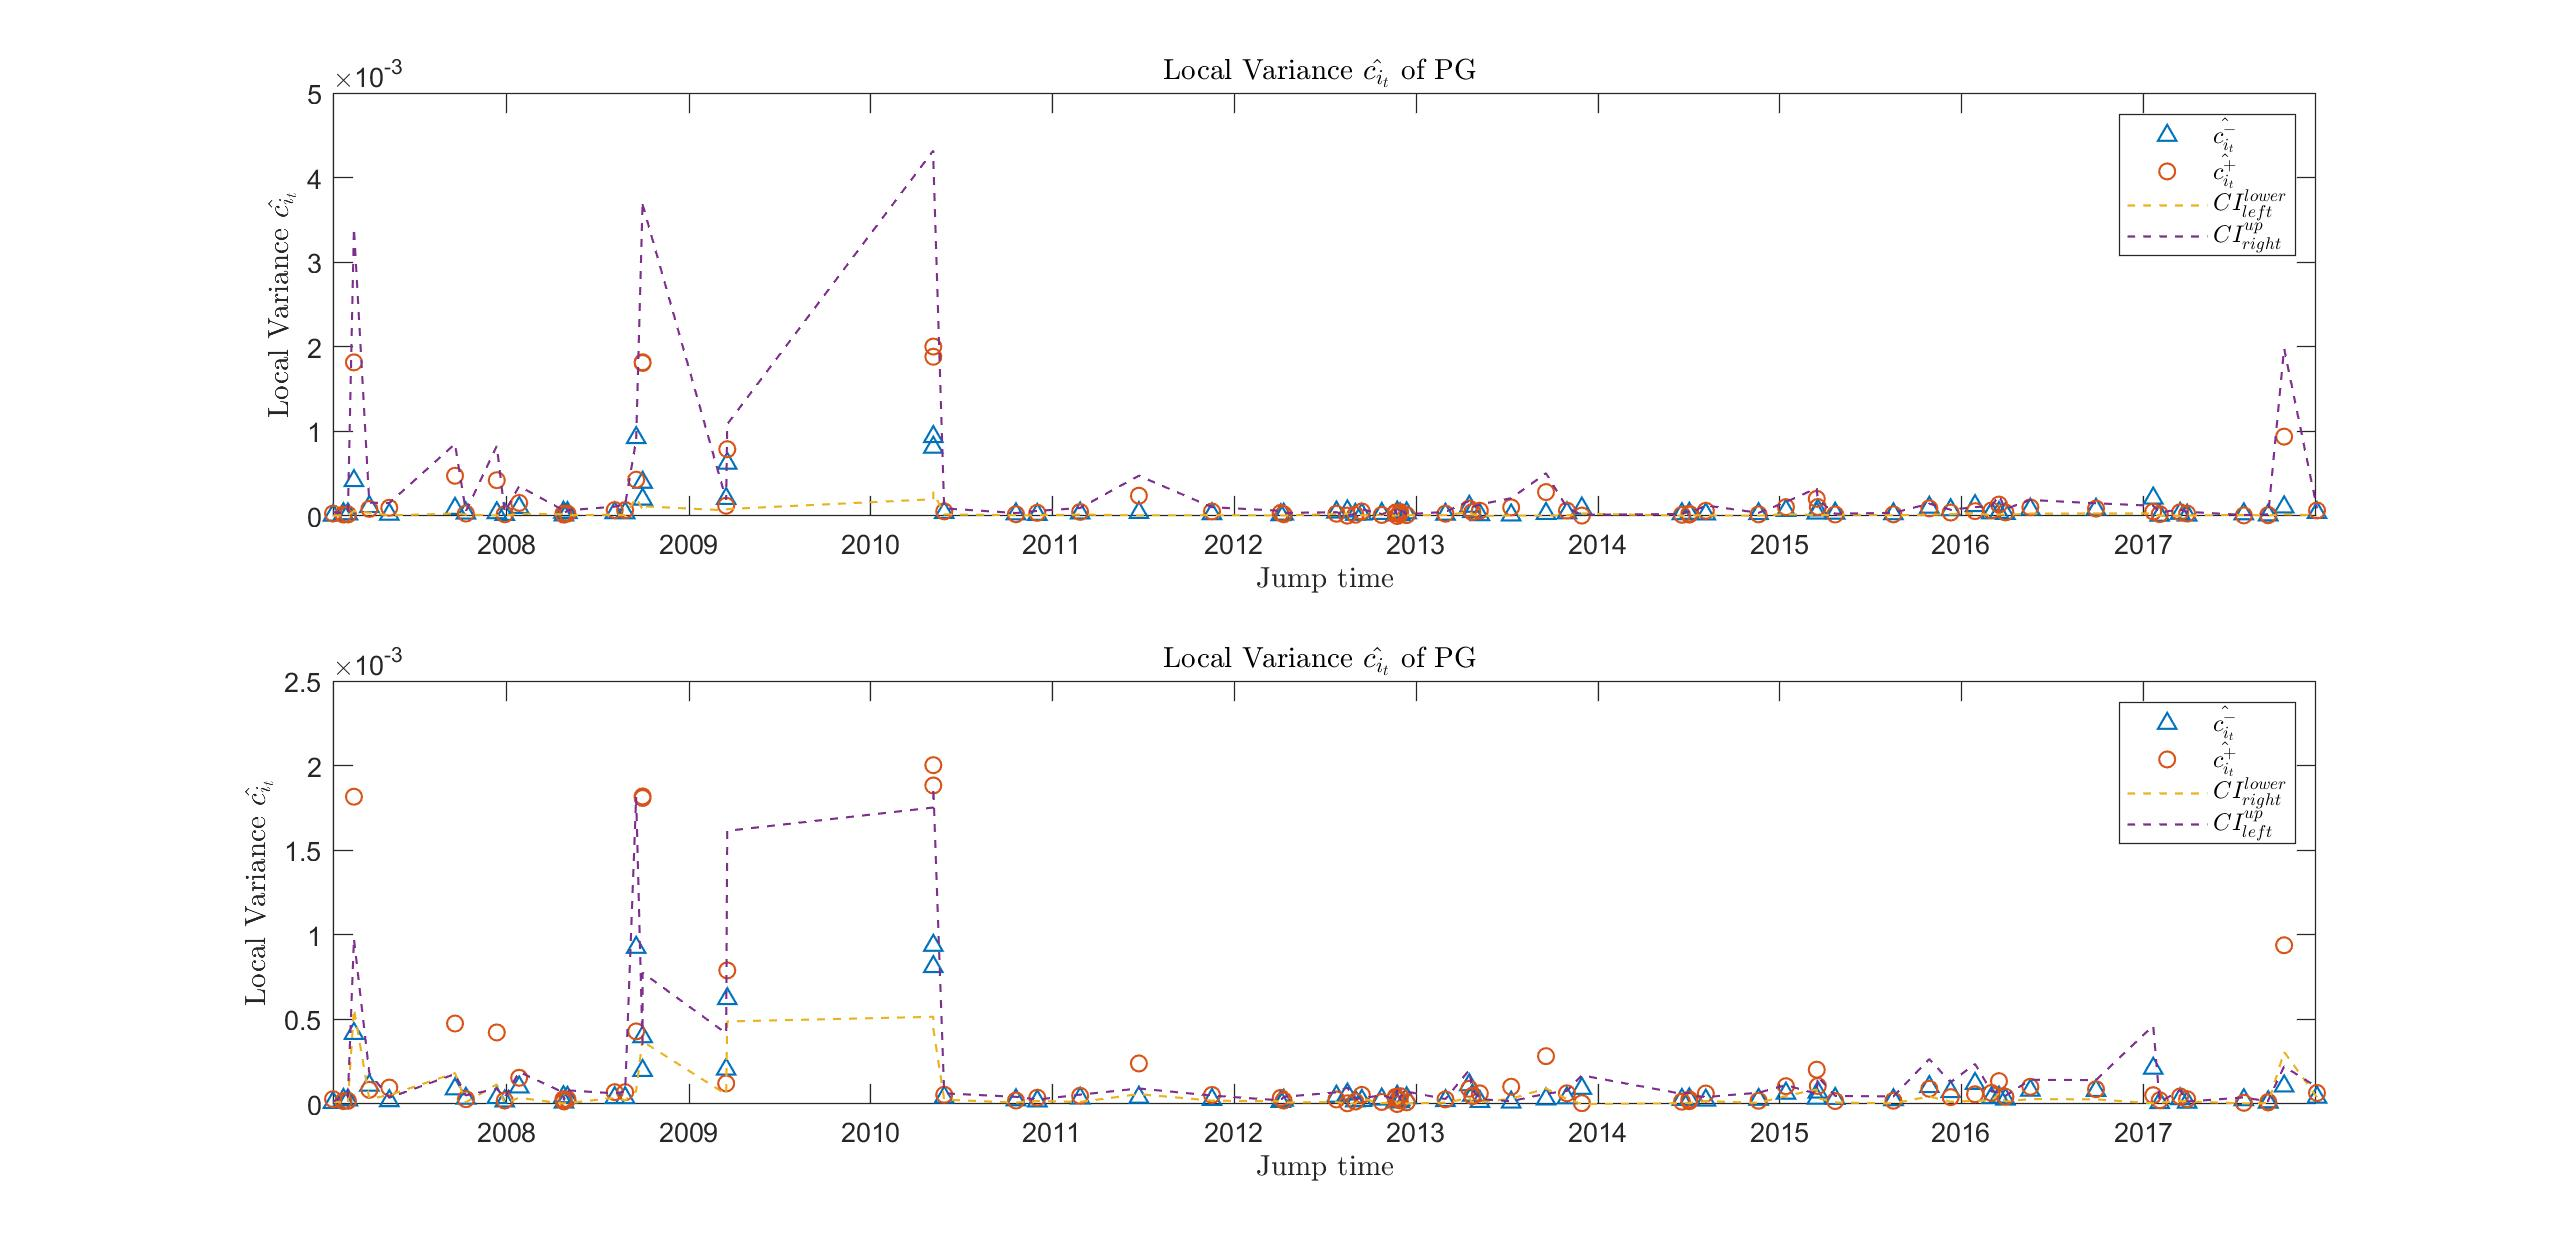
\includegraphics[width=15cm]{figures/2B_PG_2.jpg}
			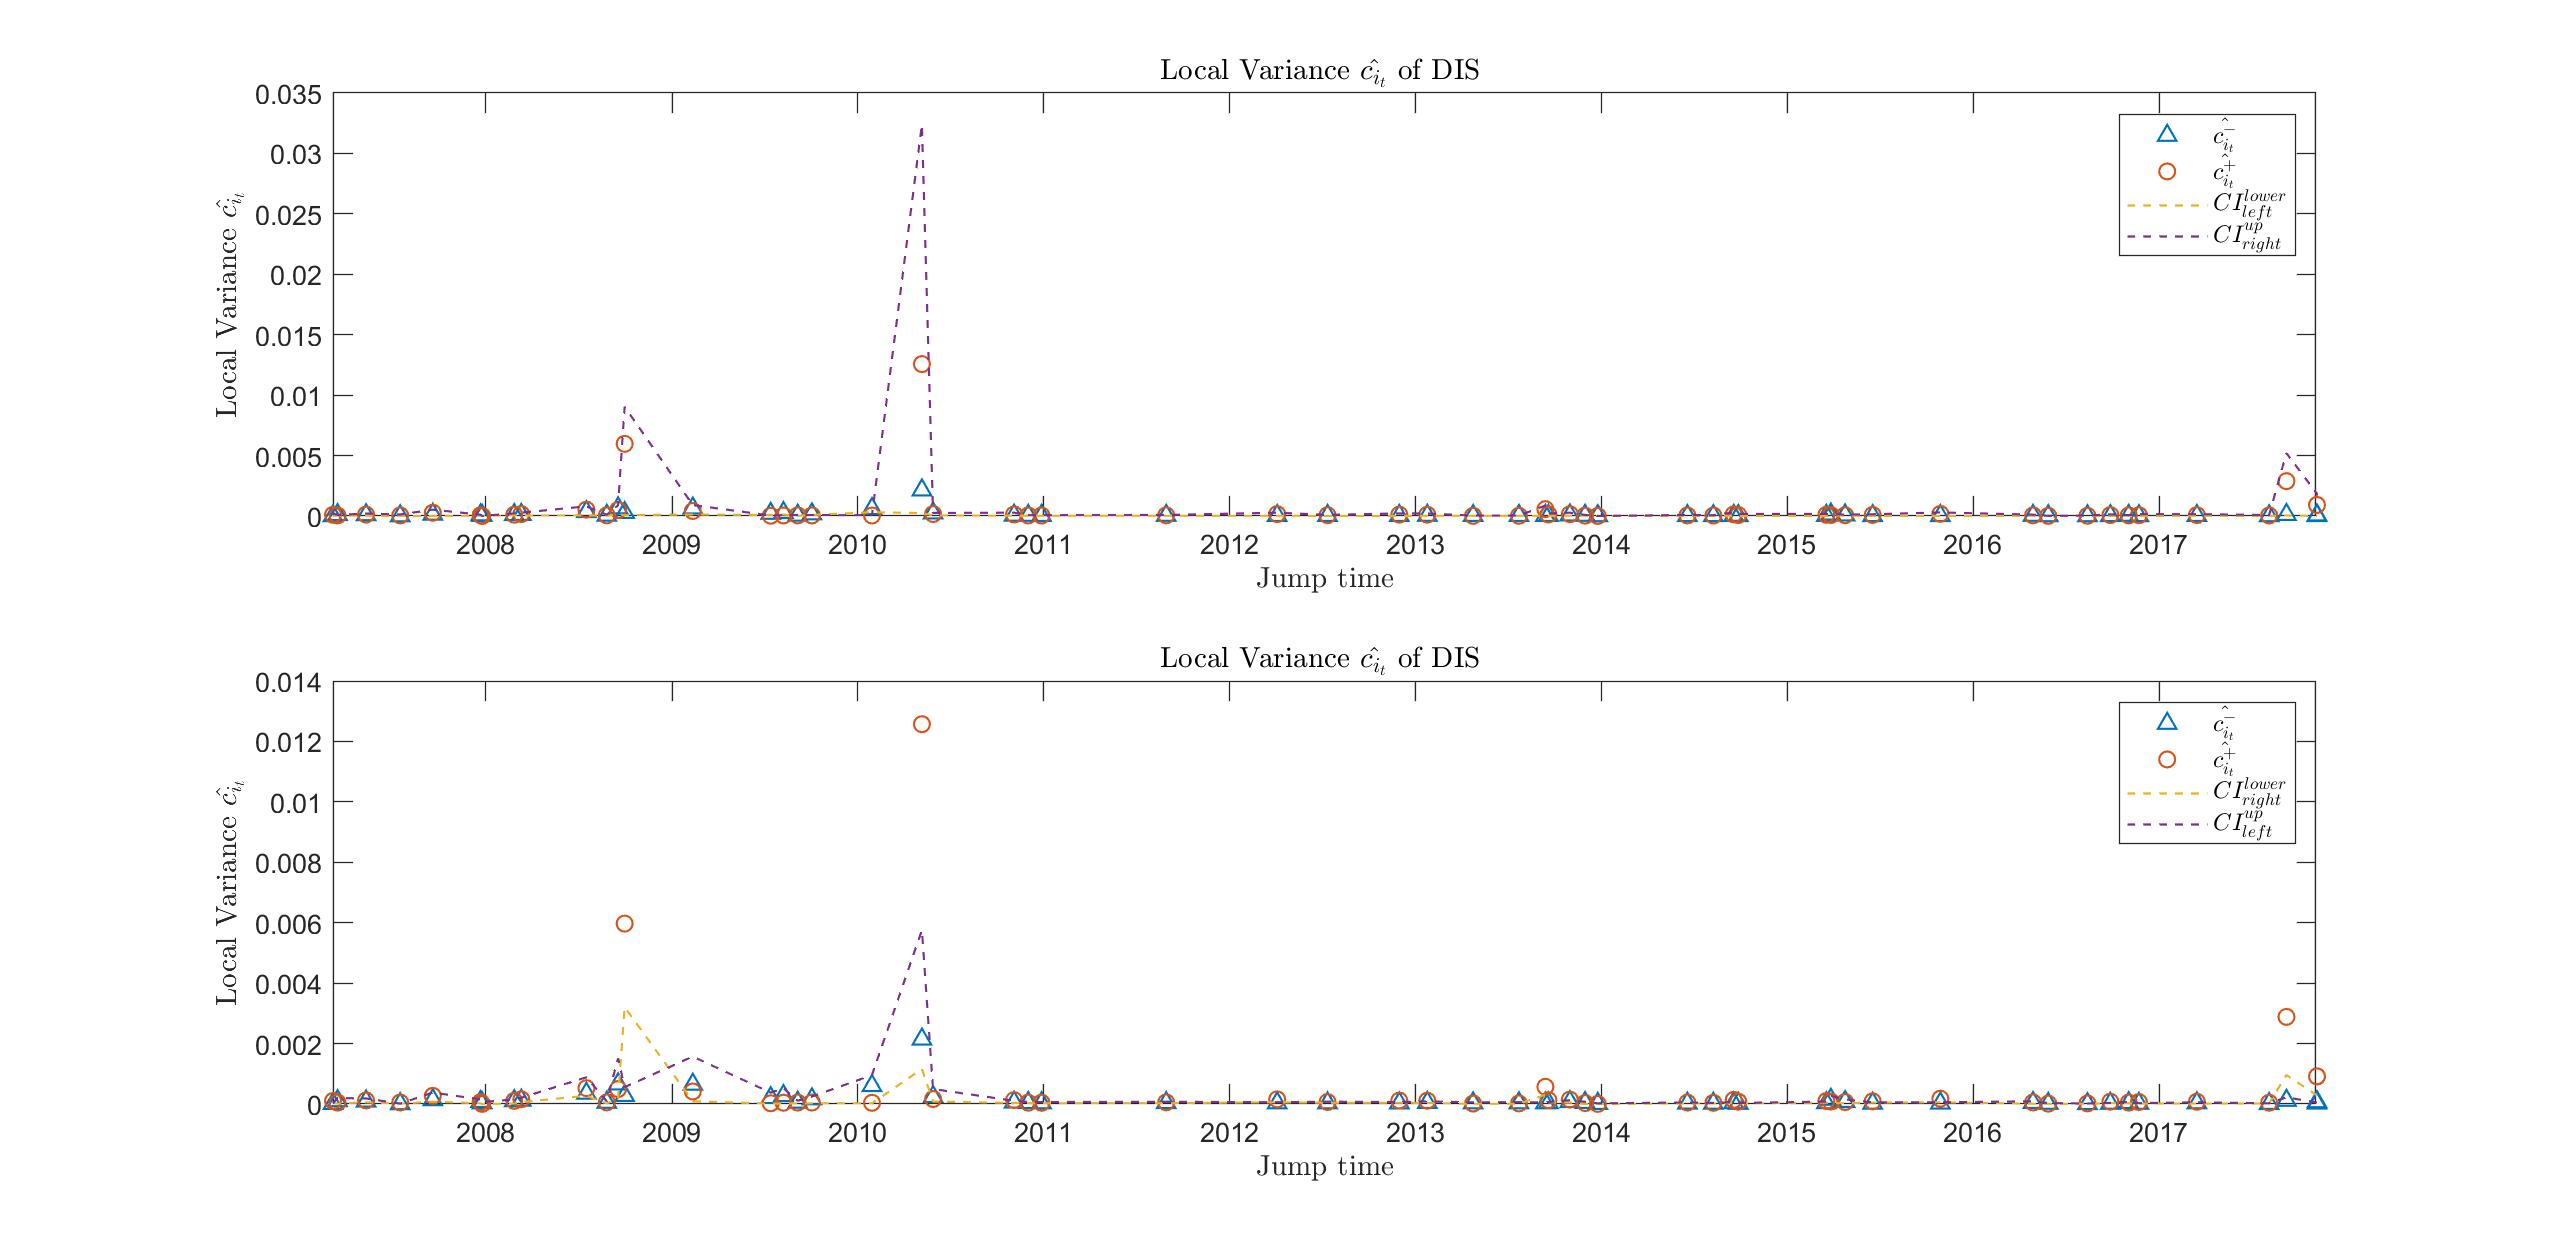
\includegraphics[width=15cm]{figures/2B_DIS_2.jpg}
		\end{minipage}
	}
	\centering
	\caption{ Mixed CI Boundary of $\hat{c}_{i_t}^-$ and $\hat{c}_{i_t}^+$ for PG and DIS}
\end{figure}

In these graphs, the purple dot lines are upper CI boundaries and the yellow dot lines are lower CI boundaries. If the lower boundaries are larger than the upper boundaries, these confidence interval of $\hat{c}_{i_t}^-$ and $\hat{c}_{i_t}^+$ will not have intersections.\\

From the graphs we can find, about 90\% of the sample data, the lower boundaries are smaller than the upper boundaries, which indicates the confidence interval of $\hat{c}_{i_t}^-$ and $\hat{c}_{i_t}^+$ will have intersections for most of time. According to our calculations, the number and percentage of intervals that do not have intersections is 14 (17.95\%) and 12 (20.69\%), for PG and DIS respectively.\\

We can put these two confidence interval together to detect their intersections more clearly.

 \begin{figure}[H]
	\subfigure{
		\begin{minipage}[l]{1\linewidth}
			\centering
			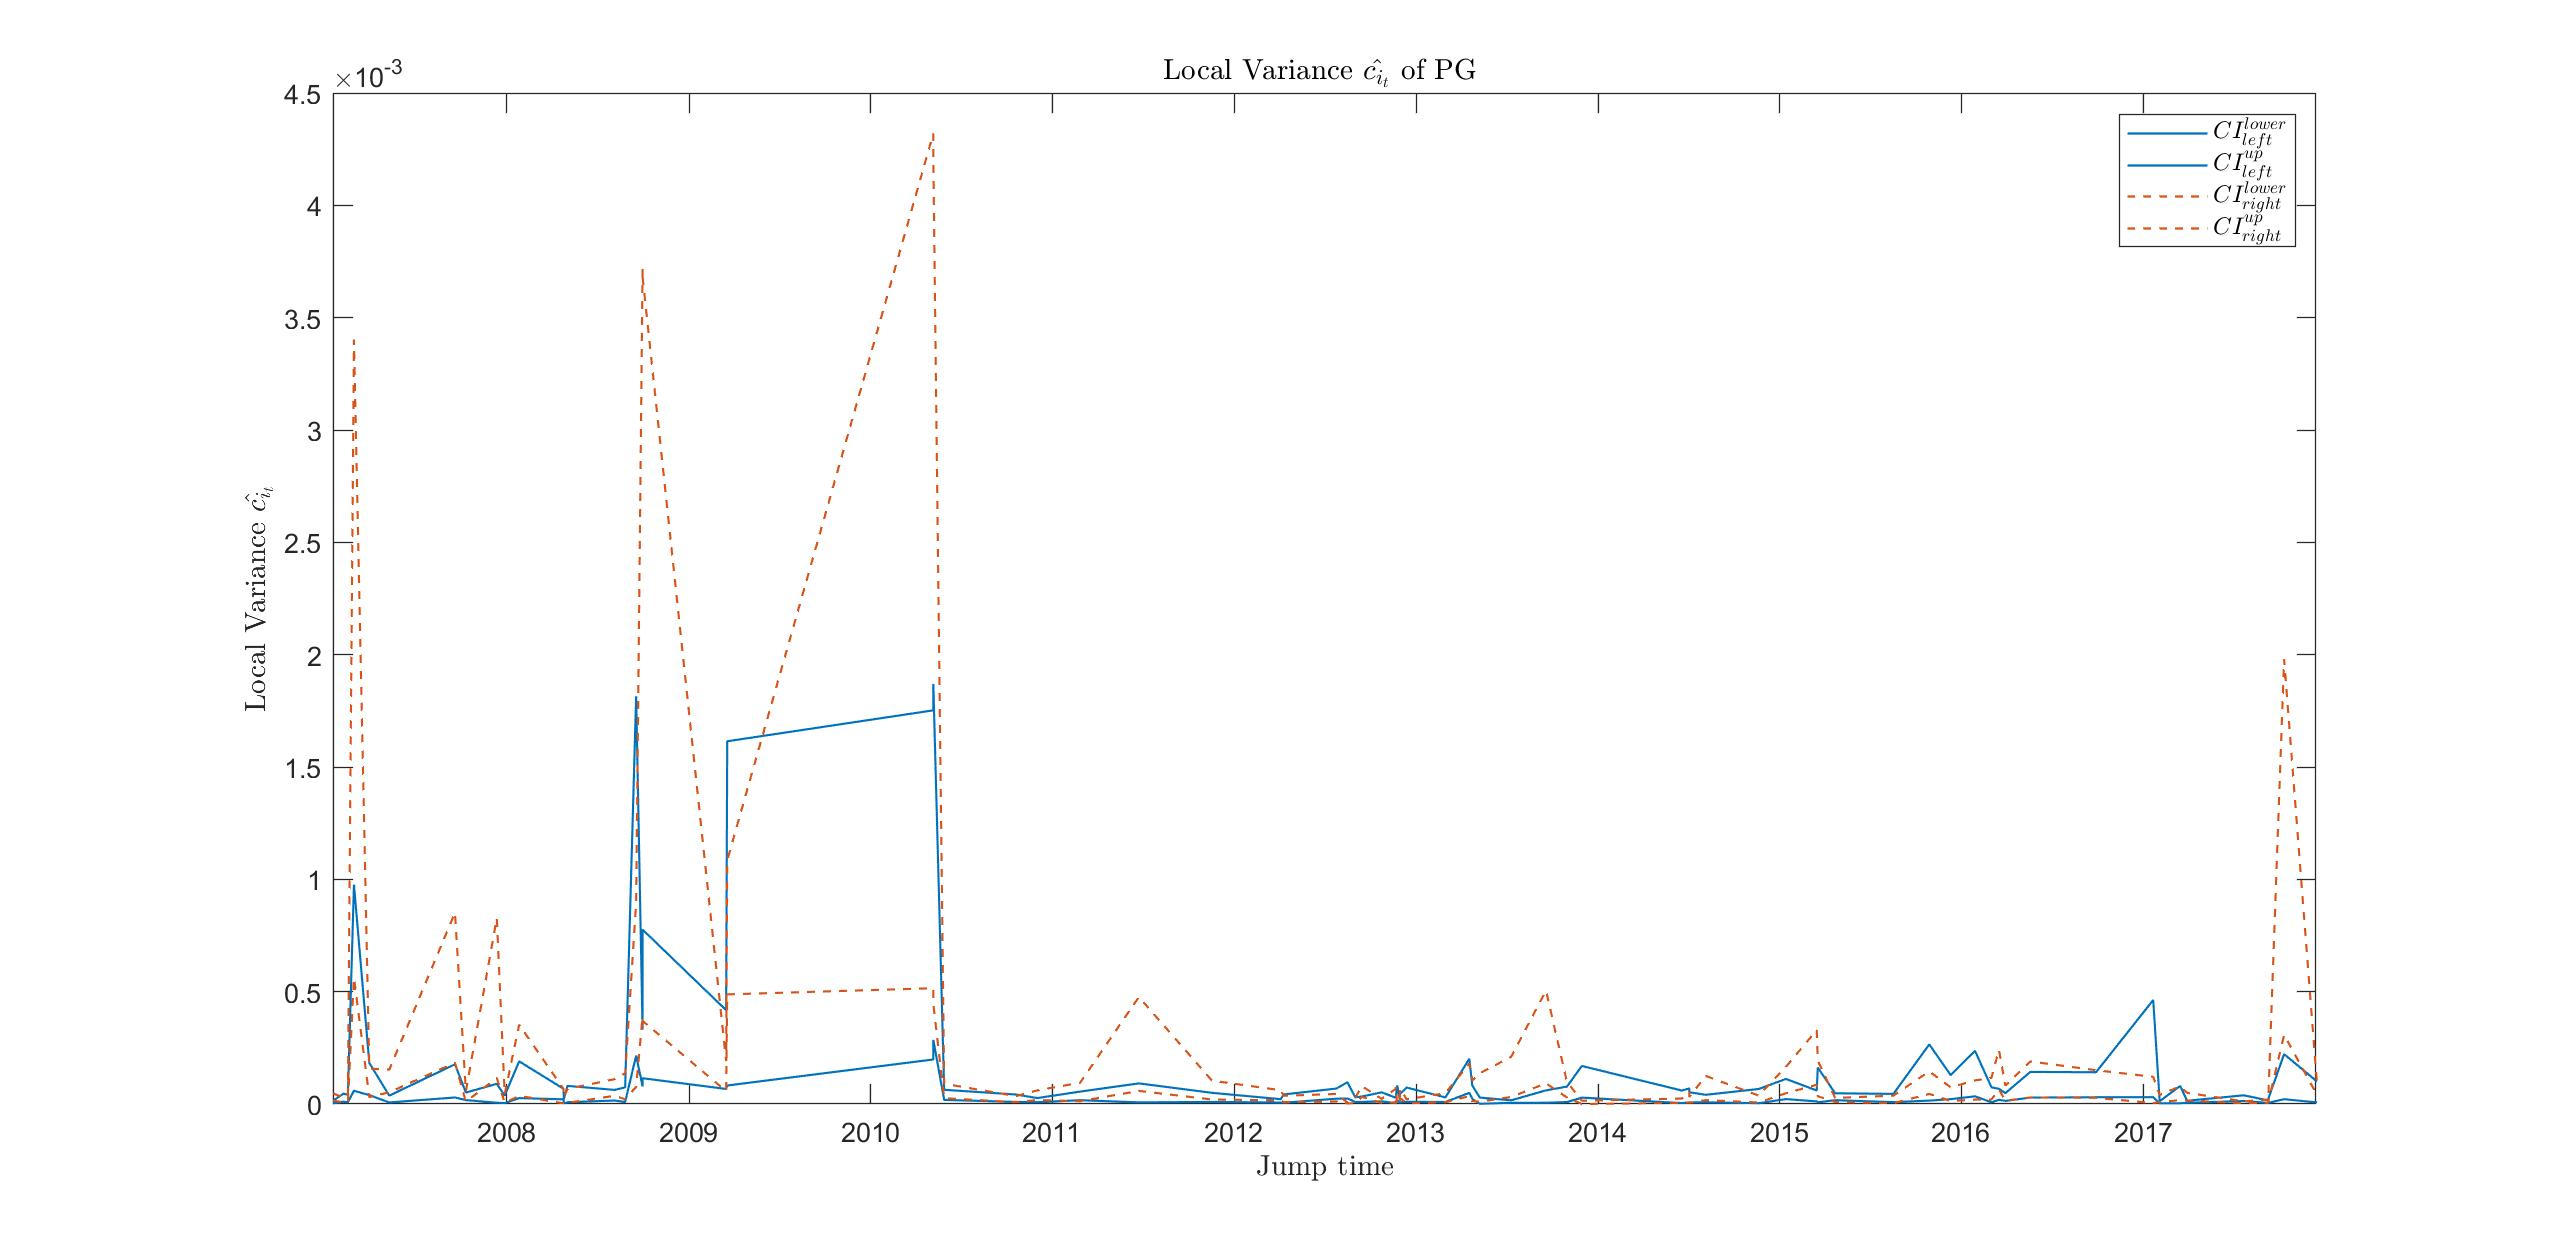
\includegraphics[width=10cm]{figures/2B_PG_3.jpg}
			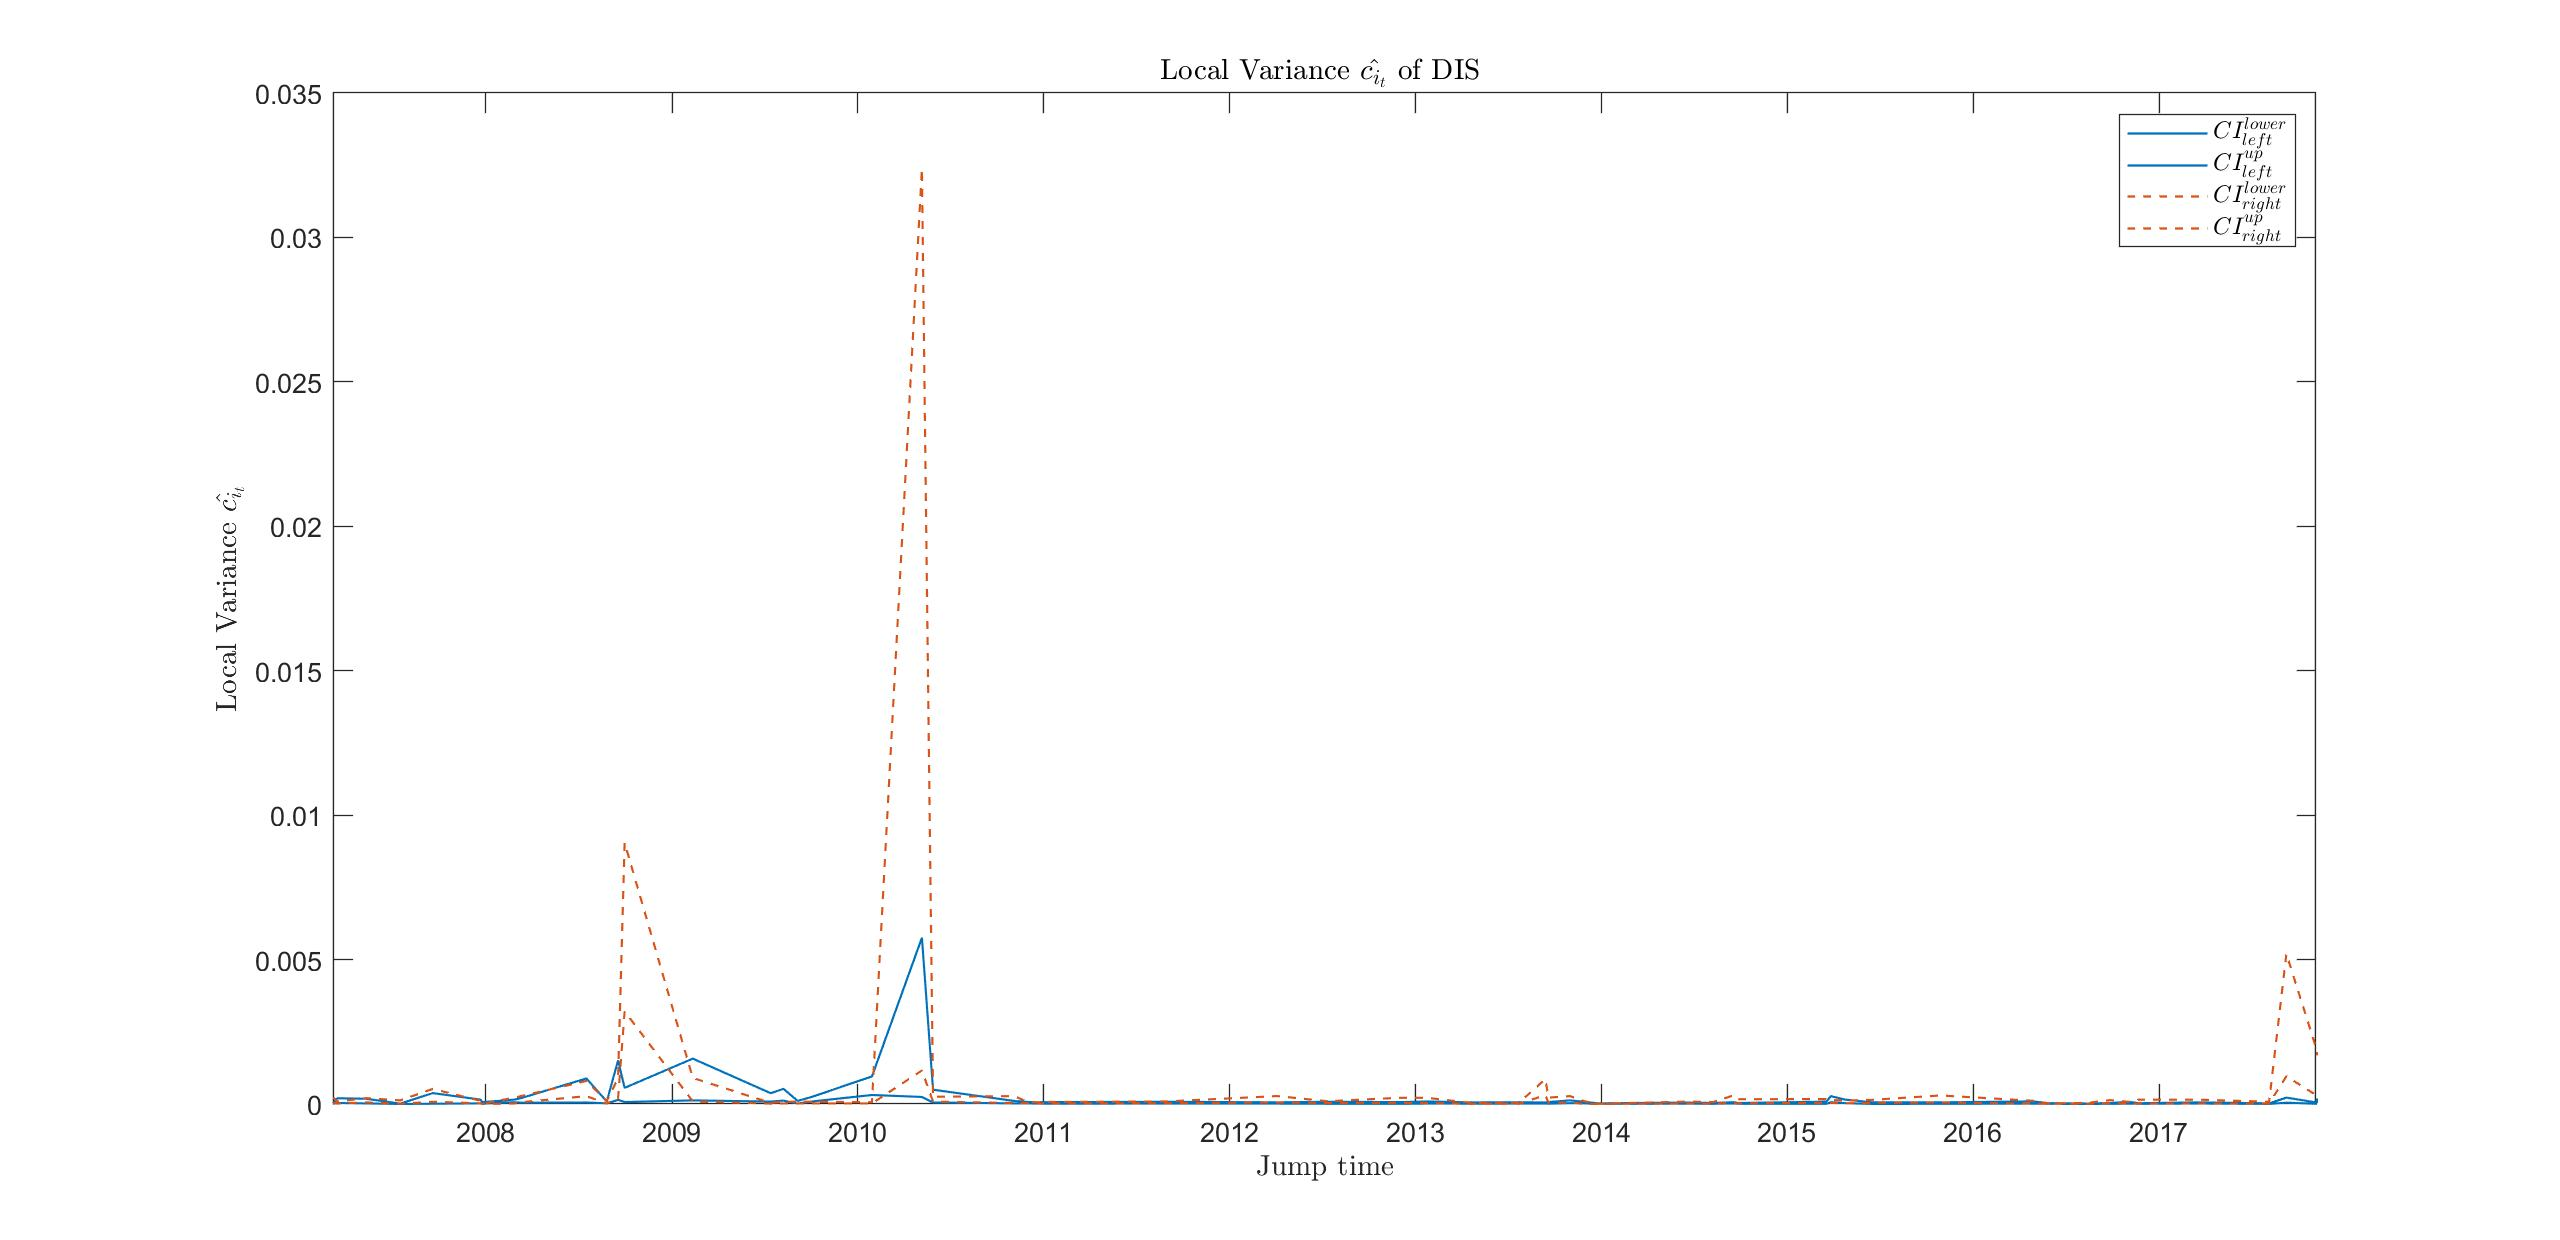
\includegraphics[width=10cm]{figures/2B_DIS_3.jpg}
		\end{minipage}
	}
	\centering
	\caption{CI Boundary of $\hat{c}_{i_t}^-$ and $\hat{c}_{i_t}^+$ for PG and DIS}
\end{figure}
The blue lines are the confidence interval of $\hat{c}_{i_t}^-$ while the red lines are the confidence interval of $\hat{c}_{i_t}^+$. Easily to see from the figures that these two confidence intervals have intersection for most of observations.\\




\end{enumerate}
The \textbf{MATLAB}:

Scripts of Q2
   \lstinputlisting{scripts/ex5_Q2_PG.m}
\end{enumerate}
\newpage

\section*{Exercise 3-Jump Regression(Jump Beta)}
\begin{enumerate}[label=\textbf{(\Alph*)}]
	%---A---
\item By using detector $I_n' \equiv \left\{i:|\Delta_i^nX_1|>\alpha\Delta_n^{0.49}\sqrt{\tau_iBV_t} \right\}$, we detect there are total 116 jumps in market log-returns. Here is the summary table sheet for jump times and return magnitude from year 2007 to 2017.

\begin{table}[ht]
	\footnotesize
		\centering % used for centering table
		\begin{tabular}{cc cccccccccc c} % centered columns (4 columns)
			\hline\hline %inserts double horizontal lines
			 Stock&2007&2008&2009&2010&2011&2012&2013&2014&2015&2016&2017\\  % inserts table
			%heading
			\hline % inserts single horizontal line
			\#Jump & 11	&5&	7	&8	&4&	17&	9&	14&	8&	18	&15 \\ 
			
			Avg.Size & 0.0047& 0.0095&0.0063 &0.0051& 0.0067& 0.0034 &0.0045& 0.0024& 0.0040 &0.0027 &0.0019 \\ %[1ex]			
			\hline %inserts single line
		\end{tabular}
\end{table}
%\vspace{-6mm}

%b
\item Here is the scatter plot of PG( and DIS)'s log-returns against the market jump returns.
 \begin{figure}[H]
	\subfigure{
		\begin{minipage}[l]{1\linewidth}
			\centering
			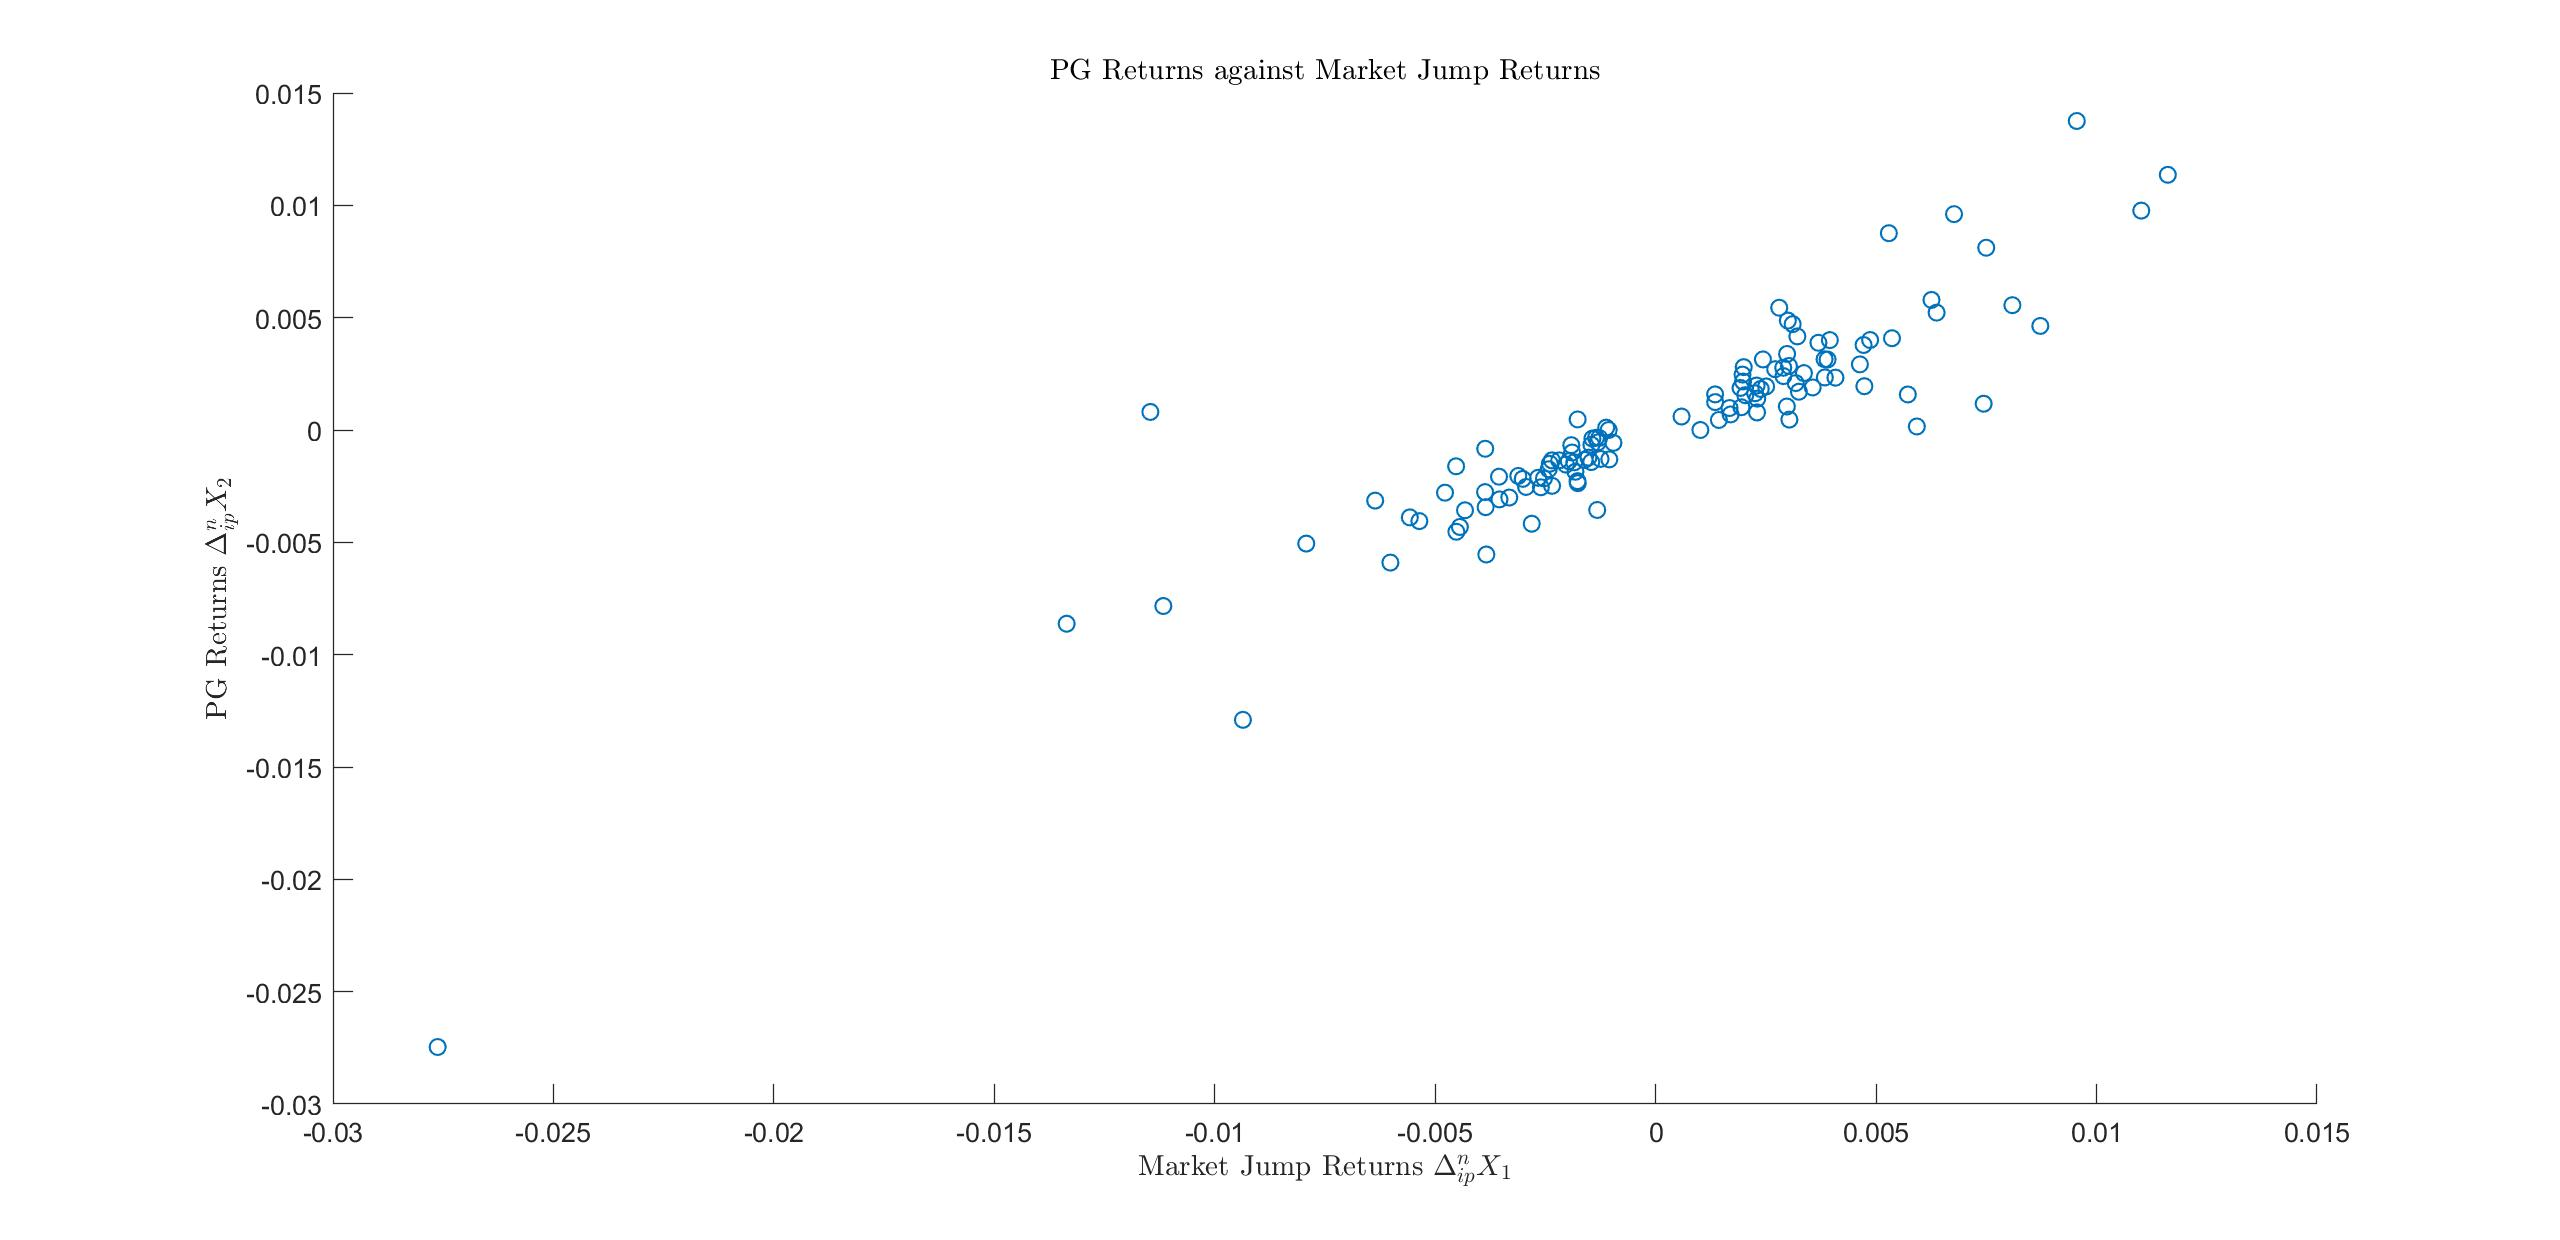
\includegraphics[width=3in]{figures/3B_PG.jpg}
			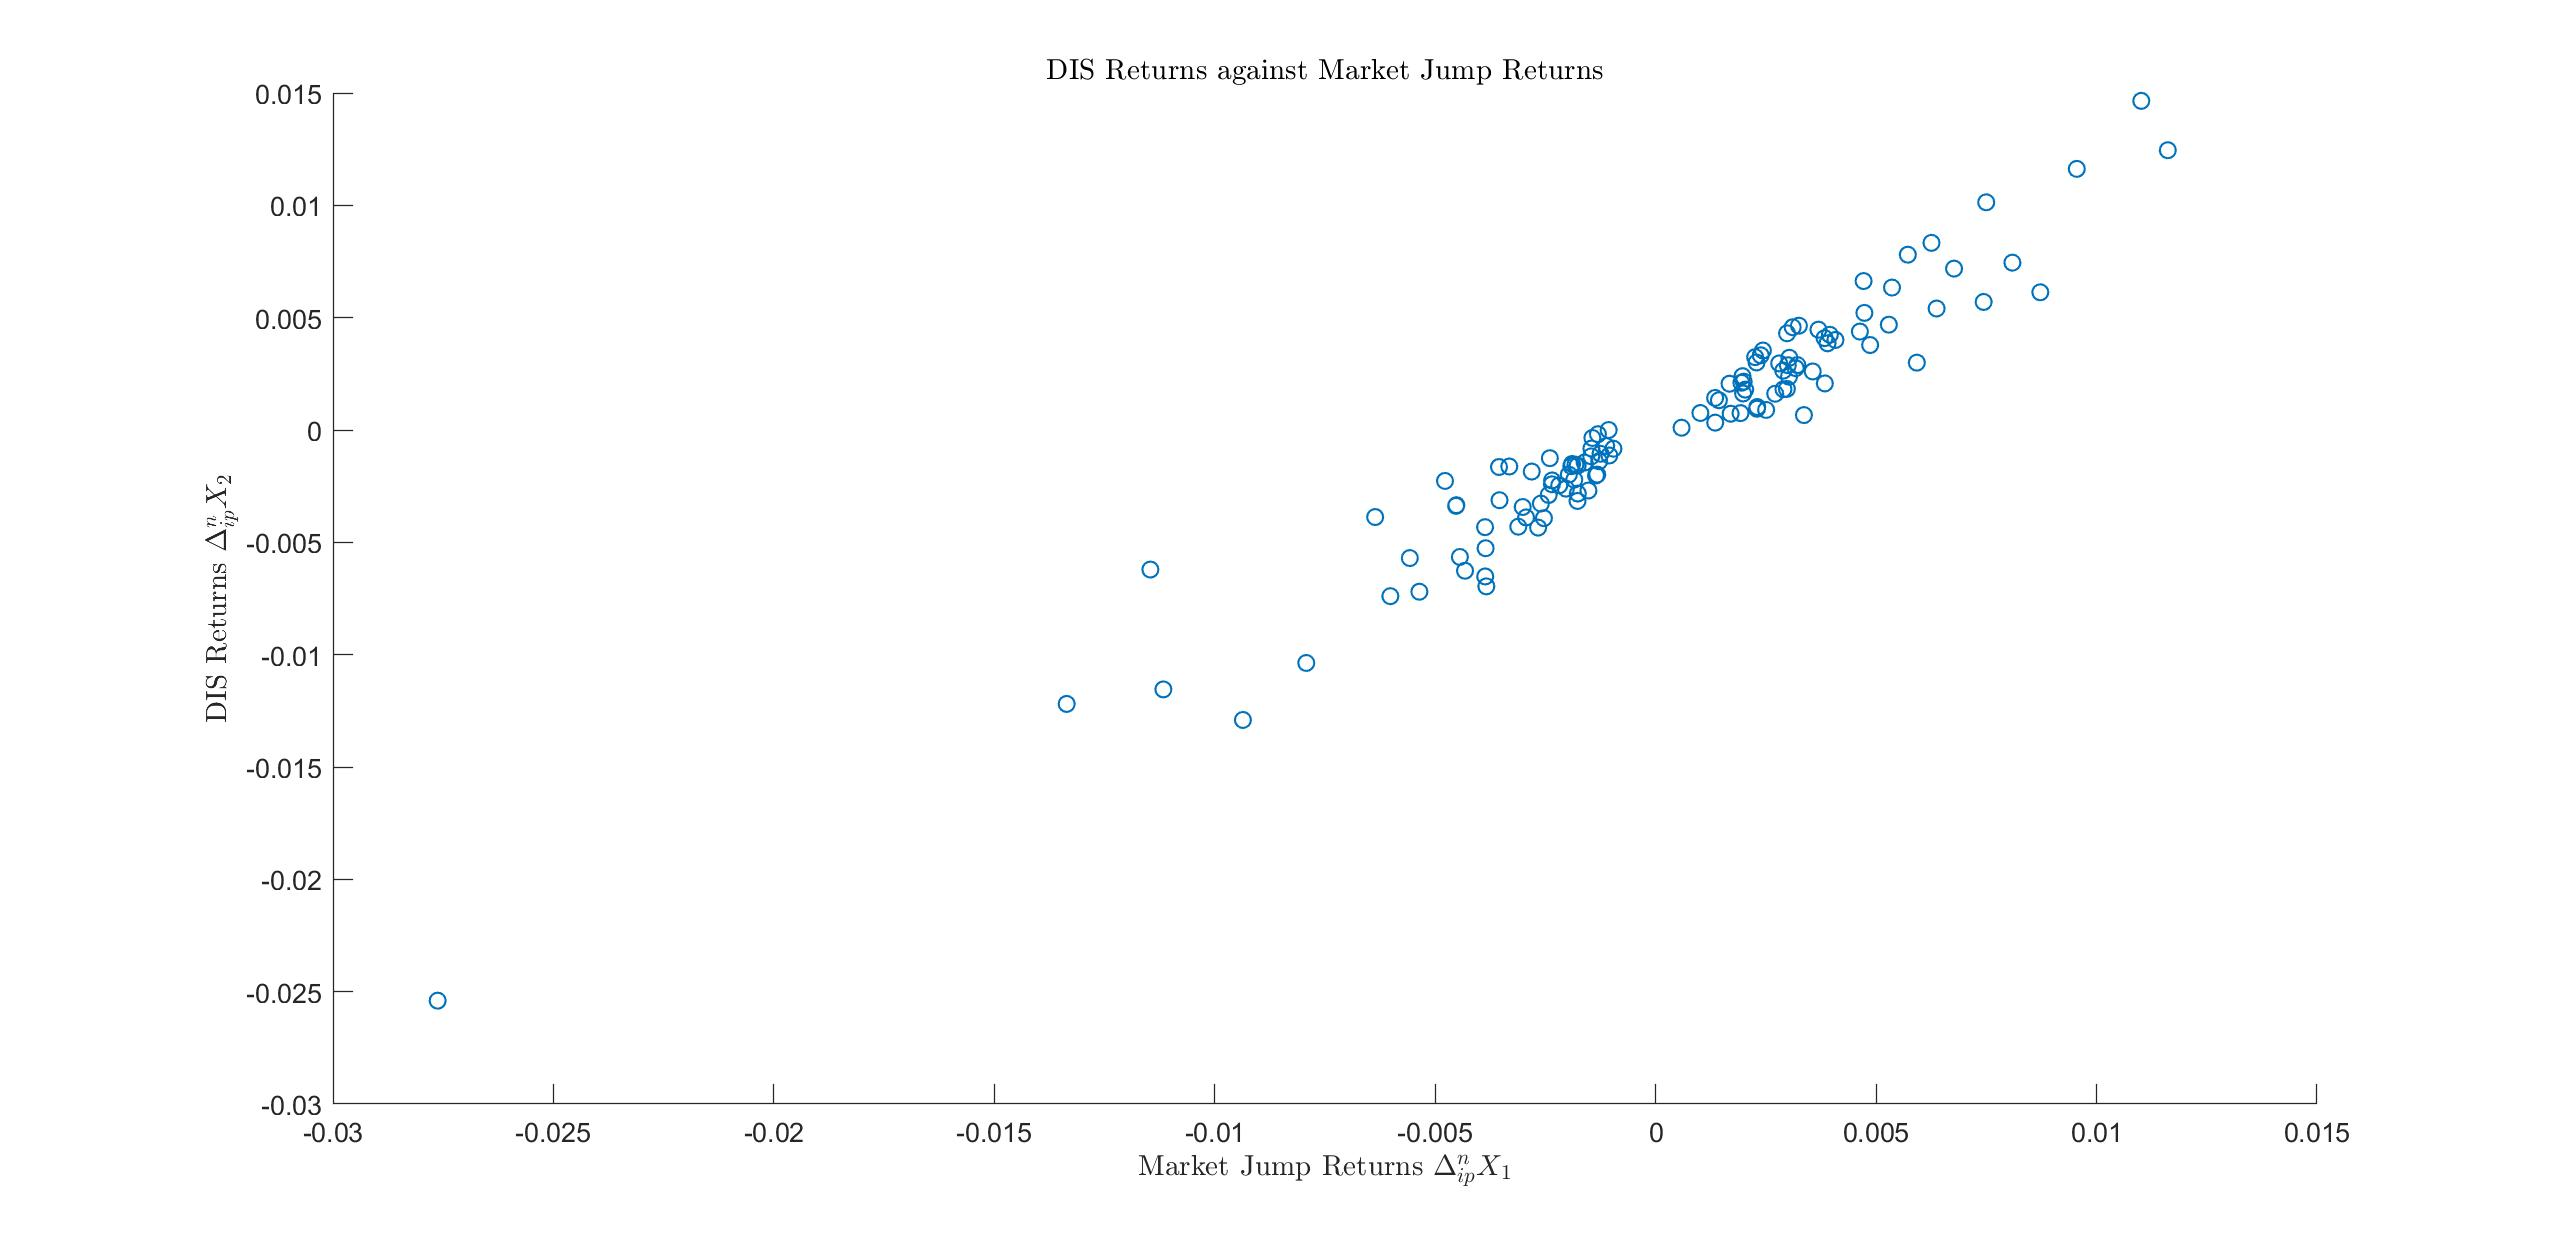
\includegraphics[width=3in]{figures/3B_DIS.jpg}
		\end{minipage}}
	\centering
	\caption{ $\hat{c}_{i_t}^-$, $\hat{c}_{i_t}^+$ and $|r_{t,i_t}^d|$ of PG and DIS}
\end{figure}
We can see, the data mostly concentrate around the origin point $(0,0)$ and the linear relationship between individual stock's log-return and market jump log-return is obvious in these figures.




%c	
\item We can get the estimator of jump beta by using the OLS regression:
$$\hat{\beta}\equiv\frac{\sum _{p=1}^{Pn}\Delta_{i_p}^nX_1\Delta_{i_p}^nX_2}{\sum _{p=1}^{Pn}(\Delta_{i_p}^nX_1)^2}$$	
 The estimate jump beta of PG and DIS:
 \begin{table}[ht]
 	\centering % used for centering table
 	\begin{tabular}{cc} % centered columns (4 columns)
 		\hline\hline %inserts double horizontal lines
 		Stock&$\hat{\beta}$\\ [0.5ex] % inserts table
 		%heading
 		\hline % inserts single horizontal line
 		PG&0.8269\\
 		DIS&0.9942\\ %[1ex]			
 		\hline %inserts single line
 	\end{tabular}
 \end{table}

Having the value of $\hat{\beta}$, we can use this regression relation to estimate out stock's returns when there is a jump in the market return:
$$Y_{stock_{i_p}}=\hat{\beta}_{stock}X_{market_{i_p}}+\epsilon_{i_p}$$
where ${i_p}$ is the detected jump time of market. The larger the $\beta$ is, the bigger jump will occur at stock's return.

\vspace{3mm}  

For PG, $\hat{\beta}=0.8269$, which means when the market return jumps for 1\%, we will expected PG's return will also experience a  jump and the jump size is   $\hat{\beta}\%$=0.8269\%. 
       
\vspace{3mm}    
          
For DIS, $\hat{\beta}=0.9942$, which means when the market return jumps for 1\%, we will expected DIS' return will also experience a  jump and the jump size is  $\hat{\beta}\%$=0.9942\%. 
 %\vspace{-6mm}
%d
\item These are the plots of stocks returns against market return with estimated regression lines.
 \begin{figure}[H]
	\subfigure{
		\begin{minipage}[l]{1\linewidth}
			\centering
			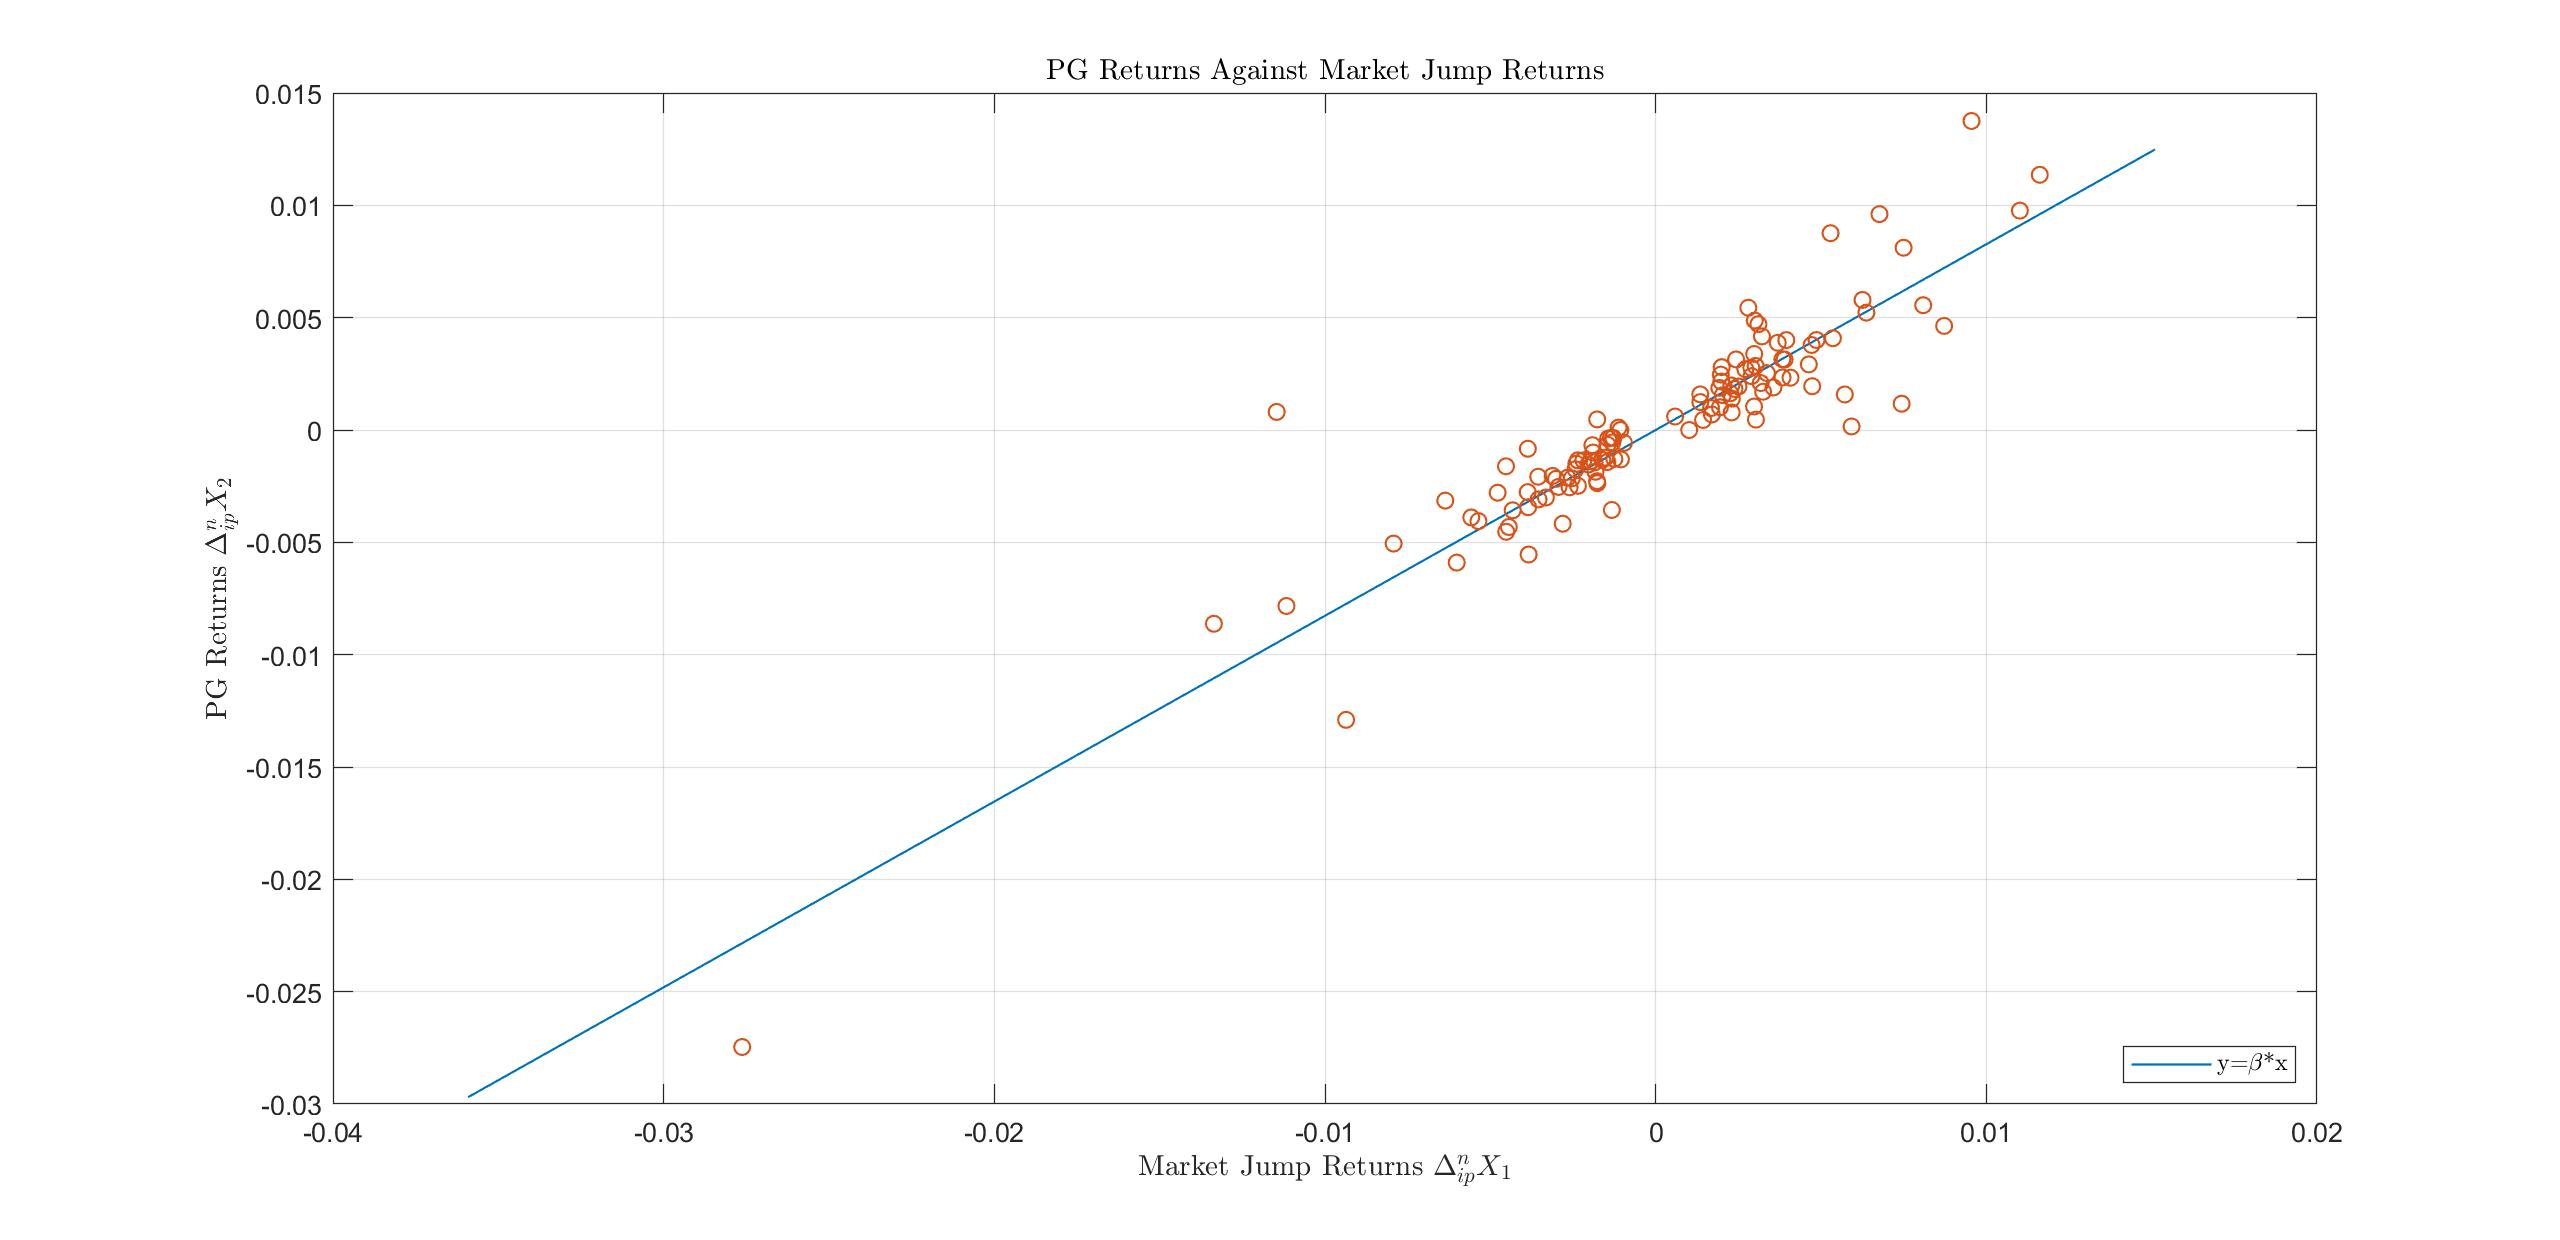
\includegraphics[width=3in]{figures/3D_PG.jpg}
			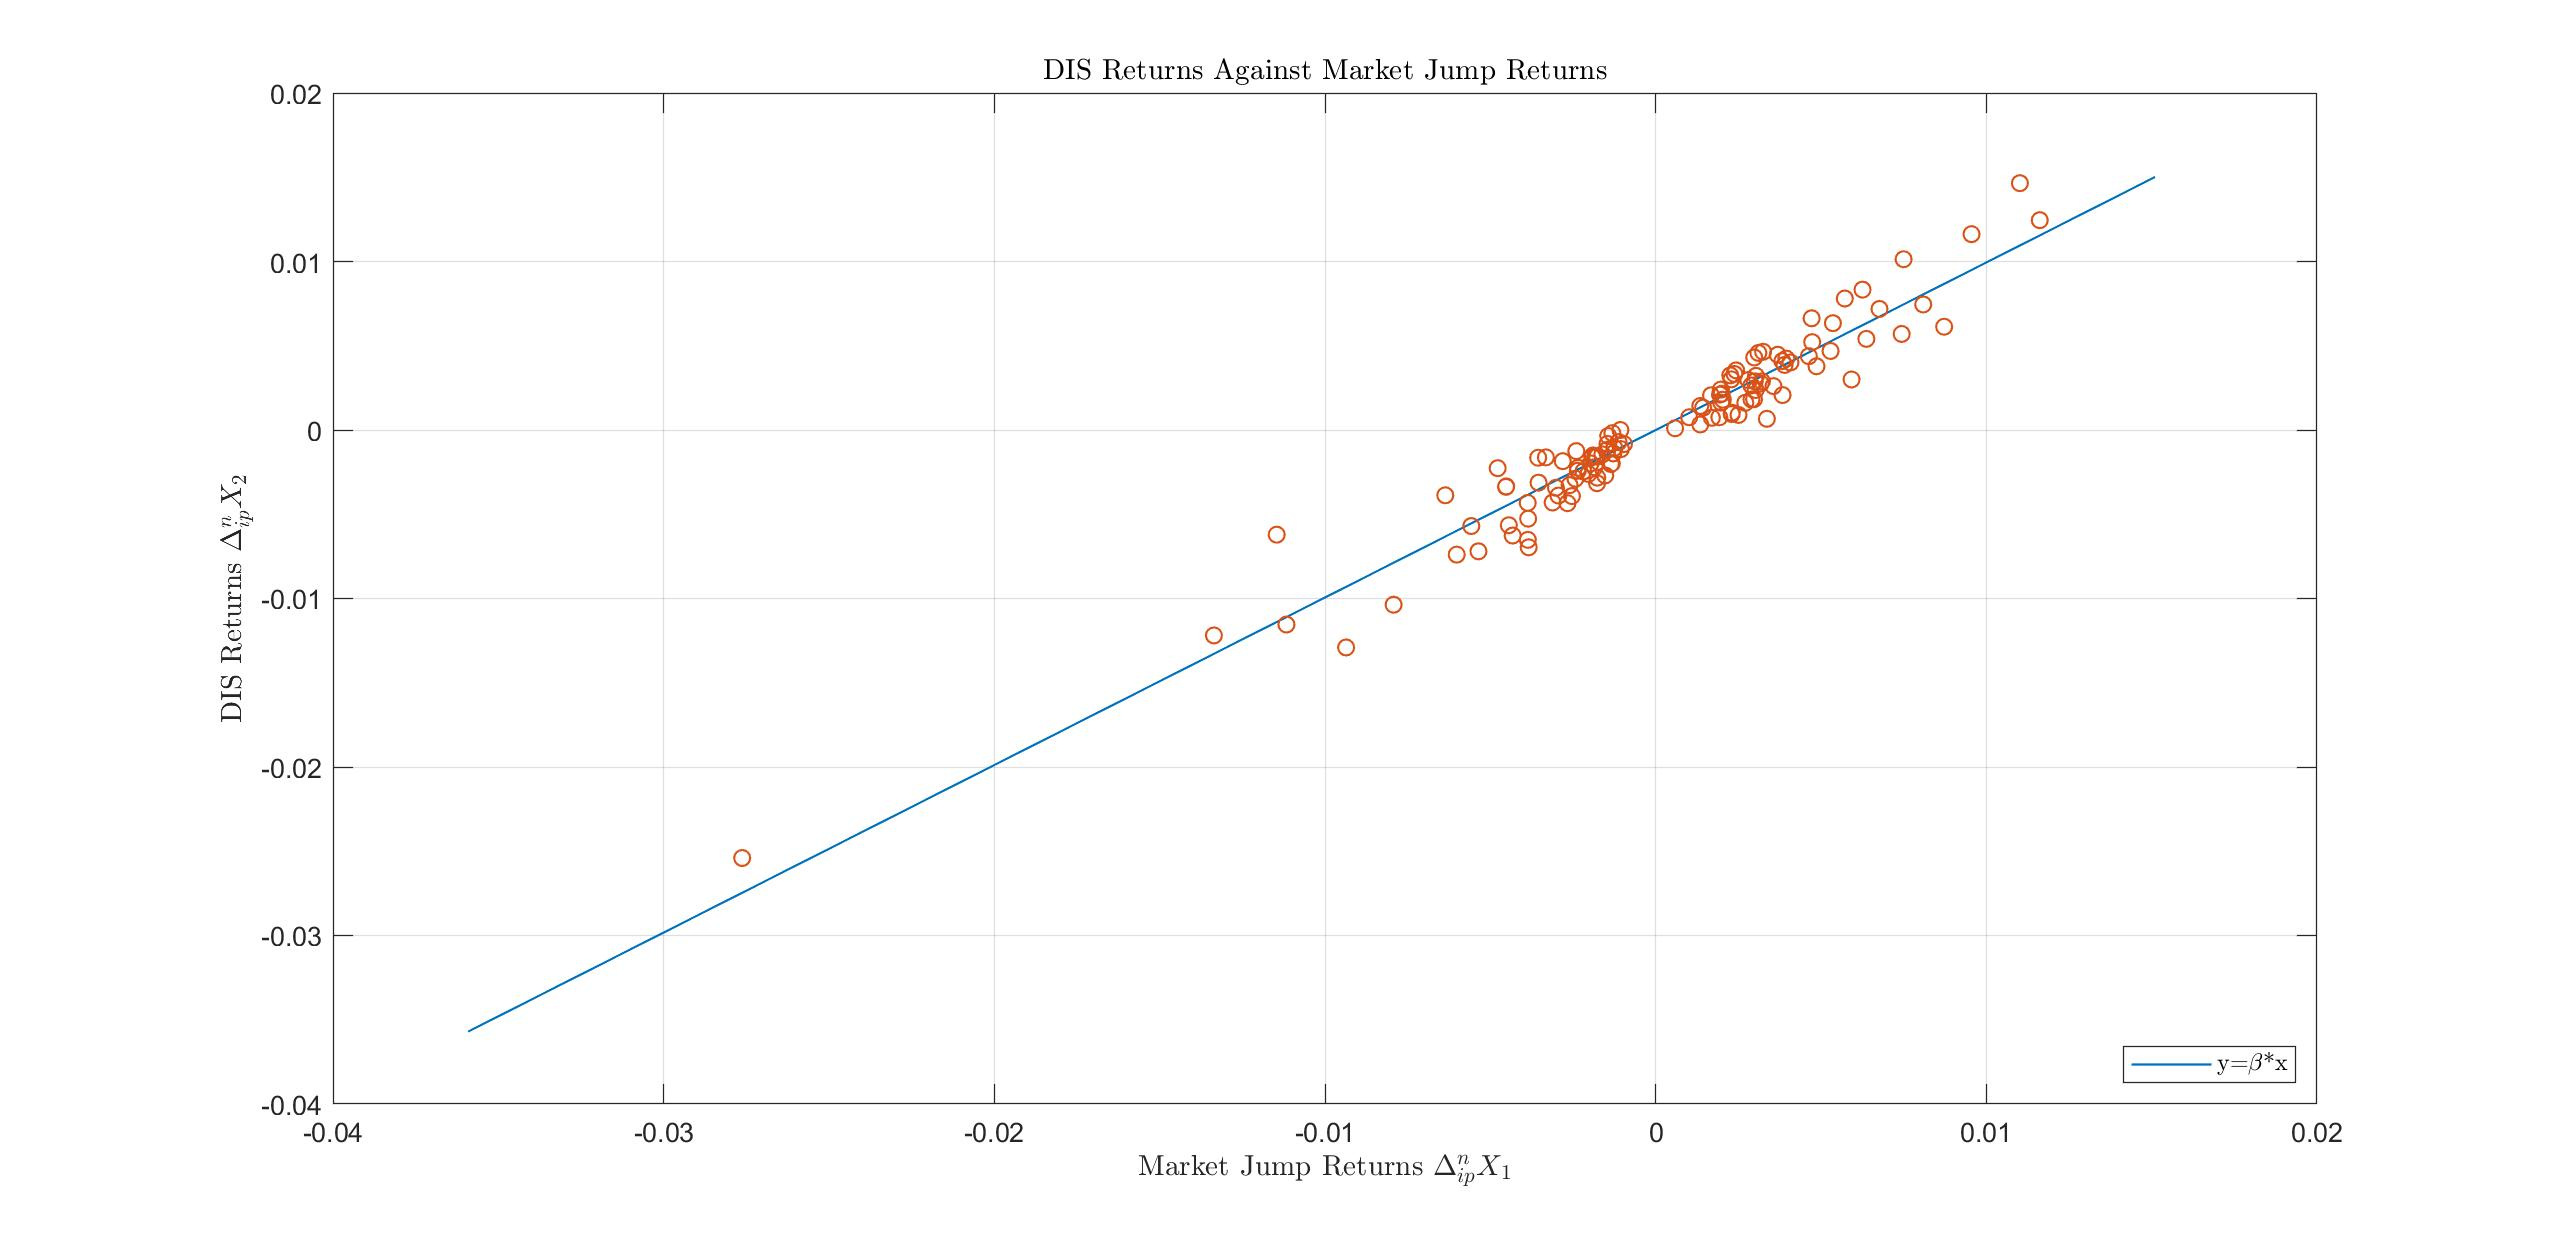
\includegraphics[width=3in]{figures/3D_DIS.jpg}
		\end{minipage}}
	\centering
	\caption{ Stock Return v.s. Market return and Regression Line}
\end{figure}

According to the graph, we can easily see the this linear regression is good since most of our data fall on or near the regression line.

%e	
\item We use this estimator to estimate the local variance for jump beta of PG and DIS:
$$\hat{V_\beta}=\frac{\sum _{p=1}^{Pn}(\Delta_{i_p}^nX_1)^2\hat{c}_{e,t_p}}{(\sum _{p=1}^{Pn}(\Delta_{i_p}^nX_1)^2)^2}$$
 
The estimated value of$\sqrt{\Delta_{i_p}^n\hat{V}_\beta}$ for PG and DIS:
\begin{table}[ht]
	\centering % used for centering table
	\begin{tabular}{cc} % centered columns (4 columns)
	\hline\hline	
		Stock&$(\Delta_{i_p}^n\hat{V}_\beta)^{\frac{1}{2}}$ \\
		\hline % inserts single horizontal line
		PG&0.0393\\
		DIS&0.0505\\ %[1ex]			
		\hline %inserts single line
	\end{tabular}
\end{table}
%\vspace{-6mm}	
%f
\item We can create a 95\% confidence interval of jump beta by using it asymptotic distribution and the confidence interval can be represented as:
$$CI_{low}=\hat{\beta}-c*\sqrt{\Delta_{i_p}^n\hat{V}_\beta}$$ 	
$$CI_{up}=\hat{\beta}+c*\sqrt{\Delta_{i_p}^n\hat{V}_\beta}$$ 
where $c=1.96$ for a 95\% confidence level interval.

The estimated 95\% confidence interval of PG and DIS.
\begin{table}[ht]
	\centering % used for centering table
	\begin{tabular}{cccc} % centered columns (4 columns)
		\hline\hline %inserts double horizontal lines
		Stock& Estimated beta & CI lower bound &CI upper bound\\
		\hline % inserts single horizontal line
		PG&0.8296&0.7499 & 0.9039\\
		DIS&0.9942&0.8952&1.0932\\ %[1ex]			
		\hline %inserts single line
	\end{tabular}
\end{table}
%\vspace{-6mm}	

For PG, the confidence interval is $CI_{\hat{\beta}_{PG}}=[0.7499,	0.9003]$, which means when there is a 1\% jump in market log-return, we will expect at lease 0.7499\% jump and at most0.9003\% jump in PG's return.

For DIS, the confidence interval is $CI_{\hat{\beta}_{DIS}}=[0.8952,	1.9032]$, which means when there is a 1\% jump in market log-return, we will expect at lease 0.8952\% jump and at most 1.9032\% jump in PG's return. Notice that $CI_{\hat{\beta}_{DIS}}$ includes the value of 1, which indices PG might perfectly co-movement with the market.

	
%g
\item  Assume you expect the market price will jump down by 1\% and $V_{stock}$ is the value of existing portfolio, $V_{mkt}$ is the value of market future index you plan to short sell, then we can use a table to show how to create a hedge strategy.
\begin{table}[ht]
	\centering % used for centering table
	\begin{tabular}{c|c|c|c|c} % centered columns (4 columns)
		\hline\hline %inserts double horizontal lines
		Asset& Position Value at $t_0$  & Position Value at $t_1$ &Cost of Position& P\&L\\
		\hline % inserts single horizontal line
		Stock&$V_{stock}$&$(1-\beta_{stock}\%)V_{stock}$ & $V_{stock}$ & $-\beta_{stock}\%V_{stock}$\\
		\hline
		Future&0&$V_{mkt}$&$(1-1\%)V_{mkt}$&$1\%V_{mkt}$\\ %[1ex]			
		\hline %inserts single line
	\end{tabular}
\end{table}

According to this table, if you want to perfectly hedge your current position, you need to short sell market index future for $V_{mkt}=\beta_{stock}V_{mkt}$, so that the P\&L for your position at time $t_1$ will equal to zero.\\

Here is the estimated short sell value confidence interval of PG and DIS:
\begin{table}[ht]
	\centering % used for centering table
	\begin{tabular}{cccc} % centered columns (4 columns)
		\hline\hline %inserts double horizontal lines
		Stock& estimated value & Value lower bound & Value upper bound\\
		\hline % inserts single horizontal line
		PG&165.3727 & 149.9728&180.7726\\
		DIS&198.8345&179.0336&218.6354\\ %[1ex]			
		\hline %inserts single line
	\end{tabular}
\end{table}
\vspace{-6mm}

%h
\item The estimated jump beta and beta variance of PG and DIS.

\begin{table}[ht]
	\centering % used for centering table
	\begin{tabular}{ccccc} % centered columns (4 columns)
		\hline\hline %inserts double horizontal lines
		Stock& $\beta_1$ & $\beta_2$ & $\hat{V}_{\beta1}$&$\hat{V}_{\beta2}$\\
		\hline % inserts single horizontal line
		PG&0.7573&0.9827&0.2784 & 0.0474\\
		DIS&0.9520&1.0957&0.4510&0.0468\\ %[1ex]			
		\hline %inserts single line
	\end{tabular}
\end{table}




\newpage
%i
\item We can create a 95\% confidence interval of $\hat{\beta_1}-\hat{\beta_2}$ by using it asymptotic distribution and the confidence interval can be represented as:
$$CI_{low}=\hat{\beta_1}-\hat{\beta_2}-c*\sqrt{\Delta_{i_p}^n\hat{V}_{\beta}}$$ 	
$$CI_{up}=\hat{\beta_1}-\hat{\beta_2}+c*\sqrt{\Delta_{i_p}^n\hat{V}_{\beta}}$$ 
where $c=1.96$ for a 95\% confidence level interval.

The estimated 95\% confidence interval of PG and DIS:
\begin{table}[ht]
	\centering % used for centering table
	\begin{tabular}{cccc} % centered columns (4 columns)
		\hline\hline %inserts double horizontal lines
		Stock& $\hat{\beta_1}-\hat{\beta_2}$  & CI lower bound &CI upper bound\\
		\hline % inserts single horizontal line
		PG&-0.2255&-0.3530 & -0.0979\\
		DIS&-0.1437&-0.3013&0.0139\\ %[1ex]			
		\hline %inserts single line
	\end{tabular}
\end{table}	



According to the table, PG's confidence interval contains zero, which means there is of 95\% probability that $\hat{V}_{\beta1}$ and $\hat{V}_{\beta2}$ are not equal.

DIS' confidence interval contains zero, which means there is a probability that DIS' $\hat{V}_{\beta1}$ and $\hat{V}_{\beta2}$ are equal. 


This result cannot be a strong evidence to against or support our assumption of jump beta is constant.\\

	The \textbf{MATLAB}:
Scripts of Q3
\lstinputlisting{scripts/ex5_Q3_PG.m}
\end{enumerate}
\end{document}
